\documentclass[12pt]{WSUThesis}
\usepackage{fullpage}
\usepackage{pslatex}
\usepackage{tabularx}
\usepackage{booktabs}
\usepackage{graphicx}
\usepackage{amsmath}
\usepackage{listings}
\lstset{basicstyle=\ttfamily, frame=single, language=python, tabsize=4}
\usepackage{tikz}
\usetikzlibrary{arrows.meta, automata, quotes, positioning, babel, shapes.geometric, arrows}


%*************** Packages *************************************

\usepackage{WSUThesis}
\usepackage{amsfonts,amsmath,amssymb,amsthm}
\usepackage{color}
\usepackage{colortbl}
\usepackage{subcaption}
\usepackage[normalem]{ulem}
\usepackage{vmargin}
\usepackage{multirow}
\usepackage{makeidx}
\usepackage[square,sort,comma,numbers]{natbib}
\usepackage[breaklinks]{hyperref}
\hypersetup{
	pdffitwindow=false,
	pdftitle={Activity Models Revisited},
	pdfauthor={Parisa Rashidi},
	pdfsubject={Dissertation},
	colorlinks=true, % false: boxed links; true: colored links
	linkcolor=black,
	breaklinks=true,
	bookmarksnumbered=true
}
\usepackage[all]{hypcap}
\usepackage{bookmark}
\usepackage{algorithm}
\usepackage{algorithmic}
\usepackage{booktabs}
\usepackage{float}
\usepackage[titletoc]{appendix}

\theoremstyle{definition}
\newtheorem{mydef}{Definition}

% redefine the input and output for algorithms
\renewcommand{\algorithmicrequire}{\textbf{Input:}}
\renewcommand{\algorithmicensure}{\textbf{Output:}}

%*************** Page Setup *************************************

\setUpThesisPages

%*************** Information *************************************

% set your information here:
\setmyname{Yuchen Hou}			  % NAME
\setmymonth{April}                  % Month degree is granted
\setmyyear{2018}                  % Year degree is granted
\setmycommitteea{Lawrence B. Holder}    % Committee Members:
\setmycommitteeb{Diane J. Cook}
\setmycommitteec{Shuiwang Ji}

\setmytitle{Link Weight Prediction with Deep Learning}					  %Title

\setmydept{School of Electrical Engineering and Computer Science} 	  % DEPARTMENT OR SCHOOL
\setmyschool{Washington State University}                             % SCHOOL
\setmydegree{Doctor of Philosophy}                                    % DEGREE TYPE
\setmythesis{Dissertation}                                            % Dissertation (Ph.D)
\setCopyright                                                        % Adds the copyright notice. Comment this line if material is not copyrighted.

%*************** Prologue *************************************

\begin{document}

% pretext pages
\DisplayTitlePage     % displays the title page with your provided information
\DisplayCopyright     % displays the copyright page with your provided information:
                      % you don't need need to comment this line even if you don't have copyrighted material. Just commenting \setCopyright suffices.
\DisplaySignaturePage % displays the signature page with your provided information
\begin{acknowledgments}
	
	Many thanks to my advisor Dr. Larry Holder for guiding and supporting me in my exploration of deep learning approaches to graph mining problems.
	This material is based upon work supported by the National Science Foundation under Grant No. 1646640.
	
\end{acknowledgments}

\begin{abstract}
	
	Deep learning has been successful in various domains 
	including image recognition, speech recognition and natural language 
	processing.
	However, the research on its application in graph mining is 
	still in an early stage.
	Here we present Model R, a neural network model created to provide a deep 
	learning approach to the link weight prediction problem.
	This model uses a node embedding technique that extracts node embeddings (
	knowledge of nodes) from the known links' weights (relations between nodes) and 
	uses this knowledge to predict the unknown links' weights.
	We demonstrate the power of Model R through experiments and compare it with 
	the stochastic block model and its derivatives.
	Model R shows that deep learning can be successfully applied to 
	link weight prediction and it outperforms stochastic block model and its derivatives by up to 73\% in terms of prediction performance.
	We analyze the node embeddings to confirm that closeness in embedding space correlates with stronger relationships as measured by the link weight.
	We anticipate this new approach will provide effective solutions to more
	graph mining tasks.
	
	We also demonstrate how to apply Model R for the collaborative rating prediction problem, which is a special case of the graph link weight prediction problem where the graph is a bipartite graph.
	This model extracts knowledge of users and items from known ratings and 
	uses this knowledge to predict unknown ratings.
	We demonstrate the power of Model R through experiments and compare it with 
	the most prevalent collaborative filtering algorithm - neighborhood-based 
	collaborative filtering.
	Model R shows that deep learning can be successfully applied to 
	collaborative rating prediction and it outperforms neighborhood-based 
	collaborative filtering by up to 18\% in terms of prediction performance.
	
	We also present Model S, a generalized deep learning approach to the graph link weight prediction problem based on general node embedding techniques.
	We evaluate this approach with three different node embedding techniques experimentally and compare its performance with stochastic block model and its derivatives.
	
\end{abstract}

% Table of contents, list of figures, list of tables
\setUpTables

%\include{./../pretext/dedicate}

%*************** Main Content *************************************
\setUpThesisStyle
\setcounter{chapter}{0}
\chapter{Introduction}
\label{chapter:introduction}

\section{Background}
Both academia and industry have seen pervasive adoption of deep learning 
techniques powered by neural network models since the early 2010s,
when they began to outperform other machine learning techniques in various 
application domains, e.g.,
speech recognition \cite{hannun2014deep},
image recognition \cite{simonyan2014very},
natural language processing \cite{yao2013recurrent},
recommendation systems \cite{barkan2016item2vec},
and graph mining \cite{grover2016node2vec}.
These neural net models not only achieve higher prediction performance than 
traditional models,
but also require much less domain knowledge and engineering.

Among those domains,
graph mining is a new and active application area for deep learning.
An important task in graph mining is link prediction \cite{liben2007link} 
\cite{al2006link}, i.e., link existence prediction:
to predict the existence of a link.
A less well-known problem is link weight prediction: to predict the weight of a link.
Link weight prediction is more informative in many scenarios.
For example, when describing the connection of two users in a social network,
a description ``Alice texts Bob 128 times per day" is more informative than
``Alice texts Bob".

Deep learning research in recommendation systems has been very active  
due to its extremely high value in industries such as search, e-commerce, 
travel and social media \cite{buettner2016predicting}.
Recommendation systems are classified into two groups according to the way they 
extract information about items: content-based filtering and collaborative 
filtering \cite{ricci2011introduction}.
Collaborative filtering extracts information from the relations between users 
and items, while content-based filtering extracts information from the contents 
of items.
There is also a hybrid approach that combines collaborative filtering and 
content-based filtering to get the strengths of both 
\cite{adomavicius2005toward}.
Collaborative filtering has multiple forms including producing a list of items 
a user would like, and predicting the ratings a user would give to a list of 
items \cite{su2009survey}.
Rating prediction as a form of collaborative filtering,
which we call collaborative rating prediction,
is in fact a special form of the graph link weight prediction problem where the graph is a bipartite graph.


We want to create a technique to predict link weights in a graph using a 
neural net model.
The model should learn to represent the graph in a meaningful way and learn to predict the target link weights using the representation it learns.

\section{Contribution}
The contribution of this thesis is
the first deep learning approach to the link weight prediction problem.
We introduce Model R - the first deep neural network model specifically designed to solve the link weight prediction problem.
We systematically study Model R's node embedding technique and illustrate its uniqueness compared to other embedding techniques.
We show that Model R significantly outperforms the state of the art non-deep learning approach to the link weight prediction problem - the stochastic block model.
We also introduce Model S - a generalized deep learning approach to the link weight prediction problem based on general node embedding techniques.
This approach requires an effective node embedding technique to produce node embeddings.
We demonstrate how this approach works with various embedding techniques including locally linear embedding \citep{roweis2000nonlinear}, and skip-gram model \citep{grover2016node2vec}.

The rest of the thesis includes the following chapters:
\begin{itemize}
	\item Problem and existing approaches: a description of the link weight prediction problem, including a social network message volume prediction example and a formal definition, and a review of the state of the art approaches to the link weight prediction problem, including Node Similarity Model, Stochastic Block Model and models derived from Stochastic Block Models.
	\item Link weight prediction with deep learning: an introduction to Model R, including its neural network architecture, node embedding technique, deep learning techniques, design parameters and choices, an experimental evaluation of the performance of Model R, with comparison to four baseline approaches on four datasets, and node embedding analysis.
	\item Model R in recommendation systems: a special use case of Model R in recommendation systems with experimental evaluations, which is a special case where the graph under analysis is a bipartite graph.
	\item Model R with pre-trained embeddings: an extension of Model R which uses embeddings produced by a generic node embedding technique.
	\item Conclusion and future work: a summary that deep learning can be applied to the link weight prediction problem and achieve better performance than the state of the art non-deep learning approaches and a brief discussion of possible future directions of this work.
\end{itemize}

\chapter{Problem and existing approaches}

\section{Problem}
We consider the problem of link weight prediction in a weighted directed graph.
We first show an example of the problem,
and then give the problem definition.
An undirected graph can be reduced to a directed graph by converting each weighted undirected link to two directed links with the same weight and opposite directions,
so the prediction for a weighted undirected graph is a special case of the problem we consider.

\subsection{Problem example}
Let us look at an example of link weight prediction, message volume prediction in a social network, shown in Figure \ref{fig:example}.
In this example, there are 3 users in a social network: A, B and C.
Each user can send any amount of text messages to every other user.
We know the number of messages transmitted between A and C, B and C, but not A and B.
We want to predict the number of messages transmitted between A and B.
\begin{figure}[!htb]\centering
	\begin{tikzpicture}[
	node distance = 4cm,
	on grid,
	> = {Stealth[length=5pt,width=4pt]},
	every state/.style = {very thick},
	every edge quotes/.style = {sloped, anchor=north}
	]
	\node[state] (B) {B};
	\node[state] (C) [below right=of B] {C};
	\node[state] (A) [above right=of C] {A};
	\path[->]   
	(A) edge["?"]   (B)
	(B) edge["7"]   (C)
	(C) edge["74"]  (A)
	(B) edge[bend left,"?"]   (A)
	(A) edge[bend left,"4"]   (C)
	(C) edge[bend left,"11"]  (B);
	\end{tikzpicture}
	\caption{
		An example of link weight prediction in a weighted directed graph -
		message volume prediction in a social network.
	}
	\label{fig:example}
\end{figure}

This is a simplified network similar to many real social networks, where every user interacts with other users by posting, sharing, following or liking them.
There can not be any logical approach to derive the unknown message volumes,
as they have randomness.
But there can be statistical approaches to build models to predict them.
The ability to predict these interactions potentially allows us to recommend new connections to users:
if A is predicted/expected to send a large number of messages to B by some model,
and A is not connected to B yet,
we can recommend B as a new connection to A.

\subsection{Problem definition}
Now we define the link weight prediction problem in a weighted directed graph.
\begin{itemize}
	\item Given a weighted directed graph with the node set V and link subset E
	\item Build a model w = f(x, y) where x and y are nodes and w is the weight of link (x, y) that can predict the weight of any link
\end{itemize}
For every possible link (1 out of $ n^2 $, where n is the number of nodes), 
if we know its weight, we know it exists;
if we do not know its weight, we do not know if it exists.
This is a very practical point when we handle streaming graphs:
for any possible link,
we either know it exists and know its weight (if it has been streamed in), or we do not know if the link will ever exist, nor know its weight.

\section{Existing approaches}
In our literature study on previous research in the link weight prediction problem,
we have found some existing approaches, but none use deep learning.
In this section,
we review these existing approaches.

\subsection{Node Similarity Model}
This approach is designed for undirected graphs.
It assumes the weight of a link between two nodes 
is proportional to the similarity of those two nodes.
It employs a linear regression model \cite{zhao2015prediction}:
\begin{align*}
w_{xy} = k \cdot s_{xy}
\end{align*}
where k is the regression coefficient,
$ w_{xy} $ is the weight of the link between node x and node y,
and $ s_{xy} $ is the similarity of x and y, calculated based on their common neighbors:
\begin{align*}
s_{xy} = \sum_{z \in N(x) \cap N(y)} F
\end{align*}
where N(x) is the set of neighbors of node x, z is any common neighbor of x and y,
and F is an index factor which has nine different forms, shown in Table \ref{tab:indexes}.
\begin{table*}[!ht]\centering
	\caption{Nine different forms of index factor F.}
	\begin{tabularx}{\textwidth}{>{\columncolor{blue!30}}cXXX}  \hline \rowcolor{blue!30}
		& Common Neighbors & Adamic-Adar & Resource Allocation \\ \hline
		Unweighted F &
		\[1\] &
		\[\frac{1}{\log(d_z)}\] &
		\[\frac{1}{d_z}\] \\ \hline
		Weighted F &
		\[w_{xz} + w_{zy}\] &
		\[\frac{w_{xz} + w_{zy}}{\log(1 + s_z)}\] &
		\[\frac{w_{xz} + w_{zy}}{s_z}\] \\ \hline
		Reliable-route Weighted F &
		\[ w_{xz} \cdot w_{zy}\] &
		\[\frac{w_{xz} \cdot w_{zy}}{\log(1 + s_z)}\] &
		\[\frac{w_{xz} \cdot w_{zy}}{s_z}\] \\ \hline
	\end{tabularx}
	\label{tab:indexes}
\end{table*}
In Table \ref{tab:indexes}, $ d_z $ is the degree of node z and $ s_z $ is the strength of node z:
\begin{align*}
s_z = \sum_{u \in N(z)} w_{zu}
\end{align*}
These nine forms represent three groups of measures of 2-hop paths connecting those two nodes:
\begin{itemize}
	\item Unweighted group \cite{adamic2003friends}:
	this group is based on path existence and ignore path weights.
	\item Weighted group \cite{murata2007link}:
	this group is based on path length, i.e., the sum of path weights.
	\item Reliable route weighted group \cite{taha1982operations}:
	this group is based on path reliability, i.e., the product of path weights.
\end{itemize}
And each group contains three forms:
\begin{itemize}
	\item Common Neighbors: this form is based on paths and ignores node degrees.
	\item Adamic-Adar: this form is similar to Common Neighbors,
	but depresses the contribution of nodes with high degrees or high strengths.
	\item Resource Allocation: this form is similar to Adamic-Adar,
	but depresses more than Adamic-Adar does.
\end{itemize}

\subsection{SBM (Stochastic Block Model)}
This approach is designed for unweighted graphs and uses only link existence information \cite{holland1983stochastic}.
The main idea is to partition nodes into L groups and connect groups with bundles.
In this way, the graph has a 2-level structure:
\begin{itemize}
	\item Lower level: each group consists of nodes which were topologically similar in the original graph
	\item Upper level: groups are connected by bundles
	to represent the original graph
\end{itemize}
Given a graph with adjacency matrix A, the SBM has the following parameters:
\begin{itemize}
	\item A: link existence matrix, where $ A_{ij} \in \{0, 1\} $
	\item z: the group vector,
	where $ z_i \in \{ 1 ... L \} $ is the group label of node i
	\item $ \theta $: the bundle existence probability matrix,
	where $ \theta_{z_i z_j} $ is the existence probability of bundle ($z_i, z_j$)
\end{itemize}
So the existence of link (i, j) $ A_{ij} $ is a binary random variable following the Bernoulli distribution:
\begin{align*}
A_{ij} \sim B(1, \theta_{z_i z_j})
\end{align*}
The SBM fits parameters z and $ \theta $
to maximize the probability of observation A:
\begin{align*}
P(A|z, \theta) 
= \prod_{ij} \theta_{z_i z_j}^{A_{ij}}(1-\theta_{z_i z_j})^{1-A_{ij}}
\end{align*}
We rewrite the log likelihood of observation A as an exponential family:
\begin{align*}
\log(P(A|z, \theta))
= \sum_{ij} (
T(A_{ij}) \eta(\theta_{z_i z_j})
)
\end{align*}
where
\begin{align*}
T(A_{ij}) = (A_{ij}, 1)
\end{align*}
is the vector-valued function of sufficient statistics of the Bernoulli random variable and
\begin{align*}
\eta(\theta) = ( \log(\frac{\theta}{1-\theta}), \log(1-\theta) )
\end{align*}
is the vector-valued function of natural parameters of the Bernoulli random variable.

\subsection{pWSBM (pure Weighted Stochastic Block Model)}
The pWSBM is designed for weighted graphs and uses only link weight information \cite{aicher2014learning}.
So it differs from SBM in a few ways described below.
Here we model link weight with a normal distribution.
Adjacency matrix A becomes the link weight matrix where the weight of link (i, j)  $ A_{ij} $ is a real random variable following the normal distribution:
\begin{align*}
A_{ij} \sim N(\mu_{z_i z_j}, \sigma_{z_i z_j}^2)
\end{align*}
$ \theta_{z_i z_j} $ becomes the weight distribution parameter of bundle ($z_i, z_j$):
\begin{align*}
\theta_{z_i z_j} = (\mu_{z_i z_j}, \sigma_{z_i z_j}^2)
\end{align*}
$ T(A_{ij}) $ becomes the vector-valued function of sufficient statistics of the normal random variable:
\begin{align*}
T(A_{ij}) = (A_{ij}, A_{ij}^2, 1)
\end{align*}
$ \eta(\theta) $ becomes the vector-valued function of natural parameters of the normal random variable:
\begin{align*}
\eta(\theta)
&= (\frac{\mu}{\sigma^2}, -\frac{1}{2\sigma^2}, -\frac{\mu^2}{2\sigma^2})
\end{align*}
The pWSBM fits parameter z and $ \theta $
to maximize the log likelihood of observation A:
\begin{align*}
\log(P(A|z, \theta))
= \sum_{ij} (
A_{ij} \frac{\mu_{z_i z_j}}{\sigma_{z_i z_j}^2}
- A_{ij}^2 \frac{1}{2\sigma_{z_i z_j}^2}
- \frac{\mu_{z_i z_j}^2}{\sigma_{z_i z_j}^2}
)
\end{align*}

\subsection{bWSBM (balanced Weighted Stochastic Block Model)}
The bWSBM is a hybrid of SBM and pWSBM
and uses both link existence information and link weight information \cite{aicher2014learning}.
The hybrid log likelihood becomes:
\begin{align*}
&\log(P(A|z, \theta))\\
=& \alpha \sum_{ij \in E} (T_e(A_{ij}) \eta_e(\theta_{z_i z_j}))\\
& + (1 - \alpha) \sum_{ij \in W} (T_w(A_{ij}) \eta_w(\theta_{z_i z_j}))
\end{align*}
where pair $ (T_e, \eta_e) $ denotes the family of link existence distributions in SBM
and pair $ (T_w, \eta_w) $ denotes the family of the link weight distributions in pWSBM.
Parameter $ \alpha \in [0, 1]$ is a tuning parameter that determines their relative importance,
E is the set of observed interactions,
and W is the set of weighted edges.
In the following, we use $ \alpha = 0.5 $ following the practice in \cite{aicher2014learning}.

\subsection{DCWBM (Degree Corrected Weighted Stochastic Block Model)}
The DCWBM is designed to incorporate node degree
by replacing pair $ (T_e, \eta_e) $ in the bWSBM with:
\begin{align*}
T_e(A_{ij}) &= (A_{ij}, -d_id_j)\\
\eta_e(\theta) &= (\log\theta, \theta)
\end{align*}
where $ d_i $ is the degree of node i \cite{aicher2014learning}.

In this chapter, we have studied the definition of the link weight prediction problem and a social network message volume prediction example. We also reviewed the state of the art approaches to the link weight prediction problem, including Node Similarity Model, Stochastic Block Model and models derived from Stochastic Block Models. Now we have a clear idea of the problem we want to solve and the existing solutions our new solution needs to outperform.

\chapter{Related work}
In this chapter, we cover the deep learning techniques developed in related work
that inspired our deep learning approach to the graph link weight prediction problem.
The biggest challenge in our research is to feed a graph to a neural network.
To tackle this challenge, we review some related work including one hot encoding, representation of words, representation of nodes and graph convolutional network.

\section{One hot encoding}
One hot encoding is a specific numeric vector representation for categorical entities.
It is a essential technique used in advanced embedding techniques such as word2vec and node2vec.
A one-hot vector is a one dimensional array which has one element set to 1 while all other elements set to 0.
In this case, the one-hot vector with nth element set to 1 represents the nth element in the category.
In a hand written digit recognition example, the input of the model is an image of a hand written digit and the output is the actual digit the image is related to.
In this case, the output is a categorical variable with 10 possible values
\[0, 1, 2, 3 ... 9\]
which can have one hot encoding as shown in Table \ref{tab:one-hot-encoding}
\begin{table}[ht]\centering
	\caption{One hot encoding for digits.}
	\begin{tabular}{cc} \hline \rowcolor{blue!30}
		Digit & One-hot encoding \\ \hline
		0 & [1, 0, 0, 0, ... 0]       \\ \hline
		1 & [0, 1, 0, 0, ... 0]       \\ \hline
		2 & [0, 0, 1, 0, ... 0]       \\ \hline
		3 & [0, 0, 0, 1, ... 0]       \\ \hline
		... & ...       \\ \hline
		9 & [0, 0, 0, 0, ... 1]       \\ \hline
	\end{tabular}
	\label{tab:one-hot-encoding}
\end{table}
This encoding scheme has its advantages compared to other encoding schemes.
For example, compared to binary encoding, output bits are completely independent from each other
so that this encoding does not introduce any false relations between different entities.

\section{Softmax regression (multinomial logistic regression)}
Softmax regression is designed to predict the value of a categorical variable.
In the digit recognition example above, when the input of the model is an image of a hand written digit,
the output should be the probability distribution over the ten possible digits
\[P(y = digit_i | x)\]
Softmax regression is commonly used as the activation function in the output layer of a neural net model to perform the final classification.
A softmax regression follows the principal that each observation in the input contributes to the probability of each category in the output. Therefore, the probability of each category in the output is a weighted sum of all the observations related to it. The weight is positive if the observation is evidence in favor of the category and the weight is negative if the observation is evidence against the category.
The math form of a softmax regression is
\[ evidence_i = \sum_j W_{i, j} x_j + b_i \]
where $ W_{i,j} $ are the weights, $ b_i $ is the bias for class i and j is the index for the observations in the input, i.e., the elements in the input vector.
The final output, probabilities y are a softmax function of the evidences
\begin{align*}
y_i
&= softmax(evidence_i) \\
&= normalize(exp(evidence_i)) \\
&= \frac{exp(evidence_i)}{\sum_k exp(evidence_k)} \\
\end{align*}
Here the softmax creates a valid probability distribution through normalization.
The exponentiation of the evidence follows the intuition that the probability of the hypothesis increases exponentially instead of linearly.
More compactly, we can use matrix multiplication to represent the softmax regression as
\begin{align*}
y
&= softmax(x) \\
&= \frac{exp(Wx + b)}{\sum_k exp((Wx + b)_k)} \\
\end{align*}
where $ y \in R^D, x \in R^d, W \in R^{D \times d}, b \in R^D $ and exp() is element wise.
Softmax units introduce nonlinearities into the model.
In a typical classification task, the value with the highest probability is regarded as the predicted value.
Some of the classification tasks require a slightly different output format: top k values, where the top k values with highest probability are regarded as the output.
The standard loss function for softmax regression is the cross entropy loss
\[loss(y, t) = - \sum_i t_i lg(y_i)\]
where y is the predicted probability distribution and t is the expected probability distribution (the one-hot encoding of the output value).
Cross entropy originates from information compressing codes in information theory.
It measures how inefficient the predicted probability distributions are for predicting the expected output value.

\section{Representations of data}
Neural nets use array representations of data exclusively in order to carry out numerical computation on the data.
The existing techniques developed for word representation in natural language processing and node representation in graph processing inspired the proposed method.
For example, a dataset representing a set of images is represented as an array with four dimensions:
\begin{enumerate}
	\item the dimension to index the image in the image set
	\item the dimension to index the row of a pixel in an image
	\item the dimension to index the column of a pixel in an image
	\item the dimension to index the color channel of a pixel
\end{enumerate}
With such a representation, an array of shape (1000, 64, 64, 3) represents a dataset of 1000 images, where each image has 64 rows and 64 columns of pixels, where each pixel has 3 color channels.
Moreover, array[3, 4, 5, 0] represent the light intensity value of image 3, row 4, column 5, channel 0.

\subsection{Representations of words}
Representations of words are very different from representations of images and audio.
Images and audio data are rich, high-dimensional data encoded as arrays of the individual raw pixel intensities for image data and power spectral density coefficients for audio data.
In image and speech recognition tasks all the available information about the entities is encoded in the data.
However, natural language data are symbolic and there is no direct way to encode words to provide useful information regarding the relationships between the symbols.
For example, images of dogs and cats illustrate their relations such as they are both four-legged, furry animals, but the words `dog' and `cat' do not illustrate these relations.

\subsection{Word2vec: word embedding with skip-gram model}
Word2vec is an efficient predictive method for word embedding. It has two variants: the Continuous Bag-of-Words model and the Skip-Gram model.
These two methods are very similar and the major difference is that the Continuous Bag-ofWords model predicts target words from context words, while the skip-gram model predicts context words from the target words \cite{levy2014dependency}.
The skip-gram model has gained popularity over time as it tends to outperform the continuous-bag-of-words model in larger datasets.
The vectors obtained from this method are very useful as features for many natural language processing tasks, such as part-of-speech tagging \cite{collobert2011natural} and named entity recognition \cite{turian2010word}.

\subsection{Node2vec: node embedding with skip-gram model}
Node2vec is a node embedding technique similar to word2vec \citep{grover2016node2vec}.
This technique reduces the node embedding problem to the word embedding problem and then applies the word embedding technique.
The most important step in this technique is to sample random walks (node sequences) from a graph.
Each random walk follows a 2nd order random walk policy: given the current node in the walk is v, the previous node in the walk is t, the unnormalized transition probability $ p(x | v, t) $ to the next node x is
\[ p(x | v, t) = \alpha(t, x) w_{vx} \]
where $ w_{vx} $ is the weight of the link (v, x), and
\begin{equation*}
\alpha(t, x) =
\begin{cases}
\frac{1}{p} &\text{if $d_{tx} = 0$}\\
1 &\text{if $d_{tx} = 1$}\\
\frac{1}{q} &\text{if $d_{tx} = 2$}\\
\end{cases}
\end{equation*}
where $ d_{tx} $ is the unweighted shortest path length from t to x (which can only be one of \{0, 1, 2\}).
The Return Parameter p controls the probability of revisiting the previous node t in the walk. With small values of p, the walk tends to go backward during the sampling process.
The In-out Parameter q controls the probability of visiting a node further away from the previous node t in the walk.
With small values of q, the walk tends to go forward during the sampling process.
The remaining probability is distributed to visiting other nodes adjacent to t.
It is a generalization of an earlier node embedding technique DeepWalk \citep{perozzi2014deepwalk}.
More specifically, DeepWalk is a special case of Node2vec where the inbound parameter p and outbound parameter q are both set to 1.
A graph has many walks, which can produce a dataset where each example is a (node, context-node) pair.
For example, given a walk in a social network of users \{John, Mary, James, Alice, Bob\}, we have the context of James \{John, Mary, Alice, Bob\}.
By reducing walks (sequences of nodes) to natural language sentences (sequences of words) and nodes to words,
this technique reduces the node embedding problem to the word embedding problem.
The final outcome is similar nodes have similar embeddings.

\section{Graph convolutional network}
Graph convolutional network is node classification technique \cite{kipf2016semi}.
It provides a method to create embeddings for graphs.
This approach is based on a localized first-order approximation of spectral graph convolutions.
The input of the model is the feature vector of the node X and the adjacency matrix of the graph A, and the output of the model is the node label Y:
\[Y = f(X, A)\]
It learns the features of nodes and local graph topologies, and represent them as the weights in its hidden layer.
The building block of a graph convolutional network is the following layer-wise propagation function:
\[H^{(l+1)} = \sigma(D^{-\frac{1}{2}} B D^{-\frac{1}{2}} H^{(l)} W^{(l)})\]
where D is a diagonal matrix:
\[D_{ii} = \sum_jB_{i,j}\]
and B is the adjacency matrix of the graph with added self-connections
\[B = (A + I)\]
where I is the identity matrix
$ H^l $ represents the activation of hidden layer l,
$ \sigma $ is the activation function, such as rectified linear unit.

In this chapter, we have studied the techniques in recent work on applying deep learning to natural language processing and graph mining.
Specifically, for deep learning techniques, we reviewed one-hot encoding, word embedding, node embedding and graph convolutional network.
Equipped with these techniques, we are ready to design a deep learning approach to the graph link weight prediction problem.

\chapter{Link weight prediction with deep learning}
In this chapter, we introduce the first deep learning approach to the graph link weight prediction problem - Model R.
We provide a detailed description of its neural network architecture, node embedding technique, deep learning techniques, design parameters and choices, an experimental evaluation of the performance of Model R, with comparison to four baseline approaches on four datasets, and node embedding analysis.

\section{Deep Learning and Embeddings}
As deep learning techniques become more powerful and standardized,
a key process of a domain-specific deep learning application
is converting entities to points in an embedding space, or equivalently,
mapping entities to vectors in a vector space,
because a neural net needs vectors as inputs.
These vectors are called embeddings and this process is called embedding.
Embeddings are ubiquitous in deep learning,
appearing in natural language processing (embeddings for words), recommender systems (embeddings for users and items),
graph mining (embeddings for nodes) and other applications.
In this section, we review a few classical embedding techniques and models for images, audio, words, documents, items and nodes.
A common goal of these techniques is to ensure that
similar entities are close to each other in the embedding space.
Observations about this process lead to our deep learning approach to link weight prediction.

\subsection{Entities and representations}
First of all, we summarize how a neural net represents various types of 
entities in different domains with different relations, as shown in 
Table \ref{tab:domains}.
An image in image recognition is represented as
a 2D light amplitude array with dimensions height and width.
An audio/spectrogram in speech recognition is represented as
a 2D sound amplitude array with dimensions time and frequency.
The relation between two images or two audio signals is not commonly included in their representations. 
Words in natural languages, items in recommendation systems, and nodes 
in graphs can be represented by vectors (1D numeric arrays).
The	relations between two words, two items and two nodes are commonly 
used to learn these vectors.
Ultimately, representations for all the entities are numeric arrays, 
because neural nets rely on neurons' activations and communications, which 
are both numeric.

\begin{table}[!ht]\centering
	\caption{
		A summary of various types of entities, their numeric
		representations and inter-entity relations in different domains.
	}
	\begin{tabular}{cccc} \hline \rowcolor{blue!30}
		Domain & Entity & Relations & Representation \\ \hline
		image recognition & image & N/A & 2D array \\ \hline
		speech recognition & audio  & N/A & 2D array \\ \hline
		natural language processing & word   & co-occurrences of words & 1D array \\ \hline
		recommendation systems & item   & co-purchases of items & 1D array \\ \hline
		graph mining & node & connections of nodes & 1D array \\ \hline
	\end{tabular}
	\label{tab:domains}
\end{table}

\subsection{Mapping entities to vectors}
The word2vec technique in natural language processing is famous for using a neural net to learn to map every 
entity (word in this case) in a vocabulary to a vector without any domain 
knowledge \cite{mikolov2013distributed}.
In a corpus, every word is described/defined only by related words in its 
contexts, by implicit relations between words in word co-occurrences.
Nonetheless, the neural net can learn from word co-occurrences and map words to 
vectors accordingly.
This approach provides strong evidence that word embedding with the Skip-gram model can extract knowledge about words from the relations between words and represent this knowledge in the word embedding space \cite{mikolov2013linguistic}.
In fact, most subsequent embedding techniques in other domains use the same Skip-gram model, such as
doc2vec \cite{le2014distributed},
item2vec \cite{barkan2016item2vec},
node2vec \cite{grover2016node2vec} and
deep walk \cite{perozzi2014deepwalk}.
All these techniques have achieved high prediction accuracies in their various applications including language modeling, document classification, item rating prediction, and node classification.

\subsection{Content-based embedding techniques}
Techniques in this group extract knowledge about an entity from its content, 
i.e., the input of the neural network is a vector produced from the item's content.
For example, the content can be the pixel values of an image, or the spectrogram of an utterance.
The similarity of these techniques is that the content (the raw input to the neural network) is already a vector.
Therefore, the embedding process is practically a dimensionality reduction process
that converts a high dimensional raw input vector to a low dimensional vector 
containing more abstract knowledge about the input entity.

\subsubsection{Image embedding with auto-encoders}
This is an unsupervised embedding technique commonly used in image recognition  \cite{vincent2008extracting}.
A small auto-encoder neural network model is shown in Figure \ref{fig:audoEncoder}.
\begin{figure}[!ht]	
	\centering
	\newcommand{\layersep}{2cm}
	\newcommand{\vocabularySize}{8}
	\begin{tikzpicture}
	[->, shorten >=1pt,node distance=\layersep]
	\tikzstyle{every pin edge}=[shorten <=1pt]
	\tikzstyle{neuron}=[circle, draw=black, minimum size=16pt, fill=green!30]
	
	\foreach \name / \y in {1,...,\vocabularySize}
	\node(input-\name) [neuron, fill=red!30, pin={[pin edge={<-}]below:}] at (\y, 0) {};	
	\node [below of=input-4, xshift = 0.5cm, yshift = 1cm] {input = the image pixel values};
	
	\foreach \name / \y in {1,...,4}
	\path[xshift=2cm]
	node(hidden1-\name) [neuron] at (\y, 1*\layersep) {};
	
	\foreach \name / \y in {1,...,2}
	\path[xshift=3cm]
	node(hidden2-\name) [neuron] at (\y, 2*\layersep) {};	
	\node [right of=hidden2-2] {embedding layer};
	
	\foreach \name / \y in {1,...,4}
	\path[xshift=2cm]
	node(hidden3-\name) [neuron] at (\y, 3*\layersep) {};
	
	\foreach \name / \y in {1,...,\vocabularySize}
	\node(output-\name) [neuron, fill=blue!30, pin={[pin edge={->}]above:}] at(\y, 4*\layersep) {};
	\node [above of=output-4, xshift = 0.5cm, yshift = -1cm] {output = the image pixel values};
	
	\foreach \source in {1,...,\vocabularySize}
	\foreach \dest in {1,..., 4}
	\path (input-\source) edge (hidden1-\dest);
	
	\foreach \source in {1,...,4}
	\foreach \dest in {1,...,2}
	\path (hidden1-\source) edge (hidden2-\dest);
	
	\foreach \source in {1,...,2}
	\foreach \dest in {1,...,4}
	\path (hidden2-\source) edge (hidden3-\dest);
	
	\foreach \source in {1,...,4}
	\foreach \dest in {1,...,\vocabularySize}
	\path (hidden3-\source) edge (output-\dest);
	\end{tikzpicture}
	\caption{
		A small auto-encoder neural network model with
		1 input layer (red), 3 hidden layers (green), and 1 output layer (blue),	input size 8, embedding size 2.
		Notice that the embedding layer is the innermost hidden layer.
		The hidden layers use rectified linear units.
		The output layer uses linear units.
	}
	\label{fig:audoEncoder}
\end{figure}
The model is a feed-forward neural network.
The output layer and the input layer have the same size.
The hidden layers closer to the input or output layers have larger sizes.
This technique is unique because during training, the input activation and the expected output activation are always the same vector of pixel values of the image.
From the input layer to the embedding layer, the layer size decreases, compressing the information.
It can effectively reduce a high dimensional vector (the activation of a large number of input units with raw pixel values)
to a low dimensional vector (the activations of a small number of hidden units with abstracted meanings)
\cite{hinton2006reducing}.
This technique applies to not only images for image recognition, but also audio spectrogram for speech recognition \cite{feng2014speech} and words for natural language processing \cite{liou2014autoencoder}.

\subsubsection{Audio embedding with convolutional neural network}
This is a supervised deep learning technique commonly used in speech recognition \cite{abdel2014convolutional}.
A small convolutional neural network model is shown in Figure \ref{fig:cnn}.
\begin{figure}[!ht]
	\centering
	\newcommand{\layersep}{1cm}
	\begin{tikzpicture}
	[->, shorten >=1pt,node distance=\layersep]
	\tikzstyle{every pin edge}=[shorten <=1pt]
	\tikzstyle{layer} = [rectangle, text centered, draw=black, fill=green!30]
	
	\node (input) [layer, fill=red!30, pin={[pin edge={<-}]below:}] {direct activation layer};
	\node [below of=input] {input = the audio spectrogram};
	
	\node (hidden1) [layer, above of=input] {convolutional layer};
	\node (hidden2) [layer, above of=hidden1] {pooling layer};
	\node (hidden3) [layer, above of=hidden2] {convolutional layer};
	\node (hidden4) [layer, above of=hidden3] {pooling layer};
	\node (hidden5) [layer, above of=hidden4] {fully connected layer};
	\node [right of=hidden5, xshift = 3cm] {embedding layer};
	
	\node (output) [layer, fill=blue!30, above of=hidden5, pin={[pin edge={->}]above:}] {fully connected layer};
	\node [above of=output] {output = the target label};
	
	\path (input) edge (hidden1);
	\path (hidden1) edge (hidden2);
	\path (hidden2) edge (hidden3);
	\path (hidden3) edge (hidden4);
	\path (hidden4) edge (hidden5);
	\path (hidden5) edge (output);
	
	\end{tikzpicture}
	\caption{
		A small convolutional neural network model with
		1 input layer (red), 5 hidden layers (green), and 1 output layer (blue).
		Notice that the embedding layer is the last hidden layer.
		The hidden layers use rectified linear units.
		The output layer uses softmax units.
		Only layers and the connections between layers are shown, while the units in each layer and the connections between units are not shown.
	}
	\label{fig:cnn}
\end{figure}
The model is a feed-forward neural network.
The input activation is the vector of pixel values of the audio spectrogram.
The output layer uses softmax units to predict the target label,
such as the genre of a song \cite{van2013deep} or the word of an utterance \cite{abdel2014convolutional}.
From the input layer upward,
each convolutional and pooling layer combo extracts more abstract information
than the previous layer.
Eventually, the neural network converts the raw input data to an embedding
at the fully connected layer and uses it to predict the target label.
Most of the studies on convolutional neural networks focus on accurately
predicting the target attributes,
and the concept of entity embedding is under-explored.
This technique applies to not only audio spectrogram for speech recognition, but also images for image recognition \cite{krizhevsky2012imagenet},
letter trigram for natural language processing \cite{collobert2008unified}
and items for recommender systems \cite{elkahky2015multi}.

\subsection{Relation-based embedding techniques}
Techniques in this group extract knowledge about an entity from its relations 
with other entities, such as words, users, items, and nodes.
The input of the neural network is the one-hot encoding vector of an entity.
The similarity of these techniques is that each entity does not contain any
information about itself and therefore its one-hot encoding vector is also
a meaningless vector.
In other words, each entity is only defined by its relations with other entities.
Therefore, in the embedding process, the neural network gradually
forms an understanding of the meaning of all entities by observing the relations
between all entities.

\subsubsection{Word embedding with skip-gram model}
This is an unsupervised embedding technique commonly used in natural language processing \cite{mikolov2013linguistic}.
A small skip-gram neural network model is shown in Figure \ref{fig:skipGram}.
\begin{figure}[!ht]
	\centering
	\newcommand{\layersep}{2cm}
	\newcommand{\vocabularySize}{4}
	\newcommand{\embeddingSize}{2}
	\begin{tikzpicture}
	[->, shorten >=1pt,node distance=\layersep]
	\tikzstyle{every pin edge}=[shorten <=1pt]
	\tikzstyle{neuron}=[circle, draw=black, minimum size=16pt, fill=green!30]
	
	\foreach \name / \y in {1,...,\vocabularySize}
	\node[neuron, fill=red!30, pin={[pin edge={<-}]below:}] (input-\name) at (\y, 0) {};
	\node [below of=input-3, yshift = 1cm] {input = word's one-hot encoding};
	
	\foreach \name / \y in {1,...,\embeddingSize}
	\path[xshift=1cm]
	node[neuron] (hidden-\name) at (\y, 1*\layersep) {};
	\node [right of=hidden-2] {embedding layer};
	
	\foreach \name / \y in {1,...,\vocabularySize}
	\node[neuron, fill=blue!30, pin={[pin edge={->}]above:}] (output-\name) at (\y, 2*\layersep) {};
	\node [above of=output-3, yshift = -1cm] {output = context-word probability distribution};
	
	\foreach \source in {1,...,\vocabularySize}
	\foreach \dest in {1,...,\embeddingSize}
	\path (input-\source) edge (hidden-\dest);
	
	\foreach \source in {1,...,\embeddingSize}
	\foreach \dest in {1,...,\vocabularySize}
	\path (hidden-\source) edge (output-\dest);
	
	\end{tikzpicture}
	\caption{
		A small skip-gram neural network model with
		1 input layer (red), 1 hidden layer (green), and 1 output layer (blue),
		vocabulary size 4 and embedding size 2.
		Notice that the embedding layer is the hidden layer.
		The hidden layer uses linear units.
		The output layer uses softmax units.
	}
	\label{fig:skipGram}
\end{figure}
The model is a feed-forward neural network.
The definition of context is the set of words close to the given word.
For example, given the natural language vocabulary \{the, quick, brown, fox, jumps, over, lazy, dog\}, the sentence ``the quick brown fox jumps over the lazy dog", a context radius of 2, and the word ``fox", we have the context of fox \{quick, brown, jumps, over\}.
A natural language corpus has many sentences,
therefore, from these sentences we can produce a dataset where each example is a (word, context-word) pair,
as shown in Table \ref{tab:words}.
\begin{table}[!ht]
	\centering
	\caption{The words dataset for a natural language corpus.}
	\begin{tabular}{cc} \hline \rowcolor{blue!30}
		Input = word & Output = context-word \\ \hline
		... & ...       \\ \hline
		brown & fox \\ \hline
		brown & jumps \\ \hline
		fox & quick \\ \hline
		fox & brown \\ \hline
		fox & jumps \\ \hline
		fox & over \\ \hline
		jumps & brown \\ \hline
		jumps & fox \\ \hline
		... & ...       \\ \hline
	\end{tabular}
	\label{tab:words}
\end{table}
Given a word ``fox'', its context word is a random variable with a probability distribution:
\[P(context\_word = x | given\_word = fox)\]
where
\[x \in vocabulary\]
and the context-word probability distribution sums to 1 over the vocabulary:
\[ \sum_{x \in vocabulary}P(context\_word = x | given\_word = fox) = 1 \]
During each training step, one training example - a (word, context-word) pair - is used.
The input layer is activated by the one-hot encoding of the given word.
The output layer is expected to predict the one-hot encoding of the context-word.
However, as each word can have many possible context-words, there is always a difference between the expected output and the actual output.
After substantial training, a skip-gram neural network model will eventually output the context-word probability distribution.
The embeddings for all words are technically the weights in the embedding layer.
For any natural language corpus and any two words X and Y in this corpus, we have the following equivalent statements:
\begin{itemize}
	\item X and Y have similar meanings
	\item X and Y have similar context-word probability distributions
	\item X and Y have similar embeddings
\end{itemize}
The final outcome is similar words have similar embeddings.
Acquiring these embeddings is often the first step in many natural language processing tasks such as paraphrasing detection \cite{socher2012deep}, constituency parsing \cite{socher2013parsing},
sentiment analysis \cite{socher2013recursive}, and
information retrieval \cite{shen2014latent}.

\subsubsection{Item embedding with skip-gram model}
This is an embedding technique similar to word embedding, commonly used in recommender systems \cite{barkan2016item2vec}.
This technique reduces the item embedding problem to the word embedding problem and then applies the word embedding technique.
For example, given a purchase order \{monitor, keyboard, mouse, printer, scanner\},
we have the context of mouse \{monitor, keyboard, printer, scanner\}.
An e-commerce platform has many purchase orders, which can produce a dataset where each example is an (item, context-item) pair as shown in Table \ref{tab:items}.
\begin{table}[!ht]
	\centering
	\caption{The items dataset for a collection of orders.}
	\begin{tabular}{cc} \hline \rowcolor{blue!30}
		Input = item & Output = context-item \\ \hline
		... & ...       \\ \hline
		keyboard & mouse \\ \hline
		keyboard & printer \\ \hline
		mouse & monitor \\ \hline
		mouse & keyboard \\ \hline
		mouse & printer \\ \hline
		mouse & scanner \\ \hline
		printer & keyboard \\ \hline
		printer & mouse \\ \hline
		... & ...       \\ \hline
	\end{tabular}
	\label{tab:items}
\end{table}
By reducing purchase orders to natural language sentences and items to words,
this technique reduces the item embedding problem to the word embedding problem.
Applying the word embedding technique will produce the desired item embeddings.
The final outcome is similar items have similar embeddings.

\subsubsection{Node embedding with skip-gram model}
This is an embedding technique similar to item embedding, commonly used in
graph mining \cite{perozzi2014deepwalk} \cite{grover2016node2vec}.
This technique reduces the node embedding problem to the word embedding problem and then applies the word embedding technique.
For example, given a walk in a social network of users \{John, Mary, James, Alice, Bob\}, we have the context of James \{John, Mary, Alice, Bob\}.
A graph has many walks, which can produce a dataset where each example is a (node, context-node) pair.
By reducing walks to natural language sentences and nodes to words,
this technique reduces the node embedding problem to the word embedding problem.
The final outcome is similar nodes have similar embeddings.

\subsection{The weakness of skip-gram model in node embedding}
The relation between nodes is quite different from that between words:
\begin{itemize}
	\item The weight of a link from one node to another specifically tells us
	how strong one node connects to the other;
	this type of relation has a regular and explicit form:
	entity - relation - entity.
	\item On the other hand, the co-occurrences of words 
	(e.g., in the context ``The quick brown fox jumps over the lazy dog")
	implicitly tells us these words are related
	but does not tell us any specific relations
	(e.g., Are ``quick" and ``brown" related? What is the relation between ``fox" and ``jumps"? Is ``over" a relation or entity?).
\end{itemize}
Natural languages do not have the notion that
all information can be described as entities and their relations, as in graphs.
For a neural net, 
words can simply show up in sequences from day-to-day conversations,
in many flexible and unpredictable ways, with little structure or regularity.
Therefore, the skip-gram model, designed to handle natural languages,
can not take advantage of highly structured data in graphs.
This suggests that a neural net, if correctly designed to handle graphs,
should be able to learn a node-to-vector mapping supervised by the link weight,
in a more specific, direct and simple way than it learns word-to-vector 
mappings supervised by word co-occurrences.

\section{Approach}
\label{model-r}
Following the above observations,
we build an estimator with a neural net model using a node pair as its input
and the weight of the link connecting the nodes as its output.
Given a weighted graph, from its adjacency list we can produce a dataset where each example is a (source node, destination node, link weight) triplet.
For example, given a social network where nodes are users and link weights are numbers of messages users send to other users, we have its adjacency list dataset as shown in Table \ref{tab:link-list-dataset}, on which we will train the model.
\begin{table}[ht] \centering
	\caption{The adjacency list dataset for a social network.}
	\begin{tabular}{cc} \hline \rowcolor{blue!30}
		\textbf{Input = (source, destination)} & \textbf{Output = weight} \\ \hline
		...                        & ... \\ \hline
		(Mary, John) & 8645 \\ \hline
		(John, Mary) & 9346 \\ \hline
		(John, Alice) & 2357 \\ \hline
		(John, Bob) & 9753 \\ \hline
		(Alice, Bob) & 1238 \\ \hline
		...                        & ... \\ \hline
	\end{tabular}
	\label{tab:link-list-dataset}
\end{table}

\subsection{Model R}
We design the model in the estimator as a fully connected neural network model which we call Model R (R as in relation), shown in Figure \ref{fig:model-r}.
We have considered a convolutional neural net as an alternative,
but we decided it would not be a good fit for this application.
The reason is that these node vectors do not have any spatial property
for a convolutional neural network to take advantage of,
compared to the 2D array of an image where the spatial location of each pixel
has significant meaning (e.g., relative distances of pixels).
These node vectors also do not have any of the invariance properties of an image,
such as translation invariance, rotation invariance,
size invariance and illumination invariance.
In this section, we describe the architecture of Model R and the node embedding technique based on this model.
\begin{figure*}[!htb]
	\centering
	\newcommand{\layersep}{1cm}
	\begin{tikzpicture}
	[->, shorten >=1pt,node distance=\layersep]
	\tikzstyle{every pin edge}=[shorten <=1pt]
	\tikzstyle{layer} = [rectangle, text centered, draw=black, fill=green!30]
	
	\node (input1) [layer, fill=red!30, pin={[pin edge={<-}]below:}] {direct activation layer};
	\node [below of=input1, xshift = -2cm] {input = (source node's one-hot encoding,};
	\node (input2) [layer, fill=red!30, pin={[pin edge={<-}]below:}, xshift = 4cm] {direct activation layer};
	\node [below of=input2, xshift = 2cm] {destination node's one-hot encoding)};
	
	\node (hidden11) [layer, above of=input1] {fully connected layer};
	\node [left of=hidden11, xshift = -3cm] {embedding layer};
	\node (hidden12) [layer, above of=input2] {fully connected layer};
	\node [right of=hidden12, xshift = 3cm] {embedding layer};
	
	\node (hidden2) [layer, above of=hidden1, xshift=2cm] {fully connected layer};
	\node (hidden3) [layer, above of=hidden2] {fully connected layer};
	
	\node (output) [layer, fill=blue!30, above of=hidden3, pin={[pin edge={->}]above:}] {fully connected layer};
	\node [above of=output] {output = link weight};
	
	\path (input1) edge (hidden11);
	\path (input2) edge (hidden12);
	\path (hidden11) edge (hidden2);
	\path (hidden12) edge (hidden2);
	\path (hidden2) edge (hidden3);
	\path (hidden3) edge (output);
	
	\end{tikzpicture}
	\caption{
		A simplified version of Model R with 1 input layer (red), 3 hidden layers (green), and 1 output layer (blue).
		Notice that the embedding layer is the first hidden layer.
		The embedding layer and the input layer both have two channels: one channel for the source node and one channel for the destination node.
		The embedding layer uses linear units
		while other hidden layers use rectified linear units.
		The output layer uses linear units.
		Only layers and their connections are shown,
		while the units in each layer and their connections are not shown.
	}
	\label{fig:model-r}
\end{figure*}
The model contains the following layers:
\begin{itemize}
	\item An input layer directly activated by the one-hot encodings of a (source node, destination node) pair.
	\item A hidden embedding layer of linear units.
	This layer maps each node from its one-hot encoding to the corresponding node vector.
	\item Multiple fully connected hidden layers of rectified linear units
	(only two layers are shown in the figure).
	These units employ the rectifier ($ f(x) = \max (0, x) $)
	as their activation function.
	These layers learn to extract more and more abstract weight-relevant 
	information.
	\item An output layer with a linear regression unit.
	This unit employs linear regression ($ f(x) = kx $) as its activation function.
	It learns to predict the link weight as a real number
	using abstracted weight-relevant information.
\end{itemize}

\subsection{Model R node embedding technique}
The Model R based node embedding technique is different from the skip-gram based techniques.
One advantage of the Model R based node embedding technique is that it takes advantage of the highly organized, regular and repeated structure in the relational dataset representing a graph, i.e., a source node connects to a destination node through one and only one weighted link.
The skip-gram model does not exploit this structure in natural language processing because this structure does not exist.
Link weights provide the information about nodes.
We fully take this property into account and design this model to learn 
complex and unobservable node information (i.e., node vectors) 
supervised by a simple and observable relation between nodes (i.e., link weight).

\subsection{Model R learning techniques}
The estimator uses the above model and a number of popular deep learning 
techniques:
\begin{itemize}
	\item Backpropagation: propagation of the error gradients from output layer 
	back to each earlier layer \cite{rumelhart1988learning}
	\item Stochastic gradient descent: the optimization that minimizes 
	the error (descending against the error gradient in weight space) for a 
	random sample in each gradient descent step \cite{lecun2012efficient}
	\item Mini-batch: the modification to stochastic gradient descent to 
	accelerate and smooth the descent by minimizing the error for a small 
	random batch of samples in each gradient descent step \cite{mairal2010online}
	\item Early stopping: the regularization used to reduce over-fitting during the iterative learning process by stopping the learning when validation error stops decreasing \cite{smale2007learning}
\end{itemize}

\subsection{Model R design parameters and choices}
Now we briefly discuss different options for our design parameters and choices,
and also some justifications for our choices.
\begin{itemize}
	\item The choice of rectifier as the activation function is a relatively easy one.
	Compared to earlier popular activation functions like sigmoid function
	($ f(x) = (1 + \exp(-x))^{-1} $),
	rectifier not only simplifies and accelerates computation,
	but also eliminates vanishing gradient problems,
	and has become the most popular activation function
	for deep neural networks \cite{lecun2015deep}.
	\item The choice of layer size is related to
	the number of examples in the dataset.
	Naturally, the larger the dataset is,
	the more discriminative the model should be,
	and consequently higher degrees of freedom,
	higher dimensions of vectors and larger layer sizes.
	Empirically, we usually set the layer size as a logarithm function of the dataset size:
	\[d = lg(n)\]
	where d (as in dimension) is the layer size and n is the number of nodes in the dataset.
	\item The choice of number of hidden layers is related to the complexity of the relation between the input and the output of the model.
	As a trivial example, if the input and the output have a linear relation,
	no hidden layer is necessary and the model is simply a linear model.
	If the input and the output have a non-linear relation,
	the more complex the relation is, the more layers are necessary.
	Empirically, we usually set the number of hidden layers to 4,
	as a good compromise of learning speed and prediction performance.
\end{itemize}
We naturally assume the most optimum design parameters are dataset dependent.
However, we do not know any theoretical way to calculate the most optimum parameters based on the statistic signatures of a specific dataset.
Therefore, in this work, we evaluate different parameter choices through experiments.
We will work on design parameter optimization in our future research.

\section{Scalability analysis}
In this section, we show that Model R has the best scalability compared to the baseline approaches. This is important when we use them in large datasets. A brief analysis shows that Model R is more suitable for prediction tasks on large streaming graphs.

\subsection{Node similarity model}
The node similarity model has two stages in its training process:
\begin{enumerate}
	\item Calculation of the node similarity for each node pair in the training set.
	\item A simple linear regression training over the training set
\end{enumerate}
The calculation of the computation complexity of the second stage is very straightforward
\[T_2 = O(e)\]
where e is the dataset size, i.e., the number of links in the graph. However, the calculation of the computation complexity of the first stage is more complicated because there are nine different forms of the similarity index factor F. Here we only estimate the Reliable route weighted resource allocation index factor because it has the highest complexity. The analysis of eight other forms of the index factor is very similar.
The first step is the calculation of the strengths of each node
\begin{align*}
	s_z = \sum_{u \in N(z)} w_{zu}
\end{align*}
where $ N(z) $ are all the neighbor nodes of $ z $ and $ w_{zu} $ are all the weights of the links connected to $ z $. This step has complexity
\[T_{1strength} = O(e)\]
where $ e $ is the dataset size, because it involves the summation of all link weights.
The second step is the calculation of the similarity for each node pair in the training set
\[s_{xy} = \sum_{z \in N(x) \cap N(y)} \frac{w_{xz} \cdot w_{zy}}{s_z}\]
where $ N(x) \cap N(y) $ are all the common neighbor nodes of $ x $ and $ y $. This step needs to iterate over all the two-hop paths in this graph so it has worst case complexity
\[T_{1similarity} = O(e^2)\]
The worst case occurs when every node is connected to every other node.
The total time complexity is the sum of the complexities of the first and second stage
\begin{align*}
	T
	&= T_{1strength} + T_{1similarity} + T_2 \\
	&= O(e) + O(e^2) + O(e) \\
	&= O(e^2) \\
\end{align*}
So the complexity is quadratic with respect to the dataset size $ v $, which is not ideal for large datasets.
Also, this model requires the presence of the entire dataset during the training due to repeated neighborhood lookup.
In other words, it needs to access the data multiple times during the training so the graph data need to be stored locally and the learning can not be done online.
This makes it difficult for the node similarity model to handle streaming graphs.

\subsection{SBM}
The SBM model's training process is to fit parameters $ z $ and $ \theta $ to maximize the probability of observation A
\[\log(P(A|z, \theta))= \sum_{ij} (T(A_{ij}) \eta(\theta_{z_i z_j})
)\]
where A is the adjacency matrix, z is the group vector and $ \theta $ is the bundle existence probability matrix.
Among these calculations, the one for A is the most complex dominating all other terms which determines the final time complexity:
\[T = O(n^2)\]
where n is the number of nodes in the graph.
We know that the number of links is always bounded by the number of nodes
\[e \leq n^2\]
Therefore we have a lower bound of the time complexity
\[T = O(n^2) \geq O(e) \]
So in the best case the time complexity is linear
\[ T = O(e) \]
And the best case occurs when the graph is fully connected.
However, many real world graphs are sparse graphs, in which case the quadratic term of the number of nodes is far larger than the number of links
\[e << n^2\]
Furthermore, the SBM model requires the presence of the entire dataset and the construction of the adjacency matrix.
Therefore, the learning cannot be done online and SBM is not suitable for streaming graphs.

\subsection{Model R}
The time complexity of a single training step is linear with respect to the number of weights/parameters in the model.
Also in a fully connected feed forward neural net layer, the number of weights is the multiplication of its number of units and the number of units in the previous layer it connects to.
Therefore, assuming each layer in Model R has the same number of units and the number of layers is a constant per the design parameter choice,
the time complexity T of Model R training is
\begin{align*}
	T
	&= O(NumberOfTrainingSteps * TimeOfEachTrainingStep) \\
	&= O(NumberOfTrainingSteps * NumberOfLayers * NumberOfWeightsPerLayer) \\
	&= O(DatasetSize * NumberOfUnitsPerLayer^2) \\
	&= O(e * lg(n)^2) \\
\end{align*}
where $ lg(n) $ is the number of units in each layer, $ n $ is the number of nodes in the graph and $ e $ is the number of links in the graph.
Most real world graphs have the number of nodes smaller than the number of links.
\[ n < e\]
Under this condition, for most real world datasets the training time complexity can be estimated by just the dataset size
\begin{align*}
	T
	&= O(e * lg(n)^2) \\
	&= O(e * lg(e)^2) \\
\end{align*}
Notice that the polylogarithmic term $ O(lg(e)^2) $ is much smaller than linear term $ O(e) $.
We can see the time complexity of the Model R is lower than those of the node similarity SBM models, which makes Model R an ideal choice for prediction tasks on very large datasets.
Furthermore, the training process of Model R does not require the presence of the entire dataset.
Instead, the training process accesses only a small subset of the dataset at a time (the mini batch of training examples) and it does not access the same data twice when the number of training epochs is set to one.
Therefore, Model R can do online learning as long as it uses each example in the training set exactly once.
This allows Model R to nicely handle streaming graphs.
In case the entire dataset is present, Model R can have multiple epochs of training.
Training with a fixed number of epochs does not change the time complexity but it may lead to over-fitting.
In the experiments, we used the technique early stopping to avoid over-fitting.
With early stopping, time complexity analysis becomes hard, because there is no way to know how many epochs will it take for the over-fitting to occur.

\section{Experiments} \label{section:experiments}
We evaluate Model R experimentally with SBM, pWSBM, bWSBM and DCWBM as baselines,
and compare their prediction errors on several datasets.
We use the same datasets and experiment process used in a recent study of these baselines \cite{aicher2014learning}.
The results show 
that Model R can achieve much lower prediction error than the baseline models.

\subsection{Datasets}
The experiments use four datasets:
\begin{itemize}
	\item Airport \cite{colizza2007reaction}. Nodes represent the busiest airports in the United States, and each of the directed edges is weighted by the number of passengers traveling from one airport to another.
	\item Collaboration \cite{pan2012world}. Nodes represent nations on Earth, and each of the edges	is weighted by the number of academic papers whose author lists include that pair of nations.
	\item Congress \cite{porter2005network}. Nodes represent the committees in the 102nd United States Congress, and each of the edges is weighted by the number of shared members.
	\item Forum \cite{opsahl2009clustering}. Nodes represent users of a student social network at UC Irvine, and each of the directed edges is weighted by the number of messages sent between users.
\end{itemize}
The statistics of these datasets are summarized in Table \ref{tab:datasets}.
\begin{table}[!ht]\centering
	\caption{
		The statistics of the graph datasets used in experiments.
		The three columns are the dataset, number of nodes, number of links and the average degree of the graph.
	}
	\begin{tabular}{cccc}  \hline
		Dataset & Node \# & Link \# & Degree \\ \hline
		Airport & 500 & 5960 & 11.92 \\ \hline
		Collaboration & 226 & 20616 & 91.22 \\ \hline
		Congress & 163 & 26569 & 163 \\ \hline
		Forum  & 1899 & 20291 & 10.68 \\ \hline
	\end{tabular}
	\label{tab:datasets}
\end{table}

\subsection{Experiment process}
We do the same experiment for each dataset.
All the link weights are normalized to the range [-1, 1] after applying a logarithm function.
Each experiment consists of 25 independent trials.
In each trial, we split the dataset randomly into 3 subsets:
\begin{itemize}
	\item 70\% into training set
	\item 10\% into validation set
	\item 20\% into testing set
\end{itemize}
A larger or smaller validation set did not reduce the prediction error in the 
experiments.
We use mean squared error as the prediction performance metric.
For each trial, the model learns for several epochs.
In each epoch,
it learns on the training set,
predicts on the validation set,
and logs the validation error.
In order to reduce over-fitting,
the estimator stops learning when the validation error has not decreased for 3 
epochs.
At the end, the testing program lets the estimator predict on the test set 
and record its testing error as its prediction error on that dataset.
For each experiment, we report the mean and standard deviation of the errors from 25 trials.

\subsection{Model prediction performance}
In our experiments,
Model R's error is lower than all other models on all datasets,
as shown in Figure \ref{fig:errors} and Table \ref{tab:errors}.
\begin{figure*}[!ht]\centering
	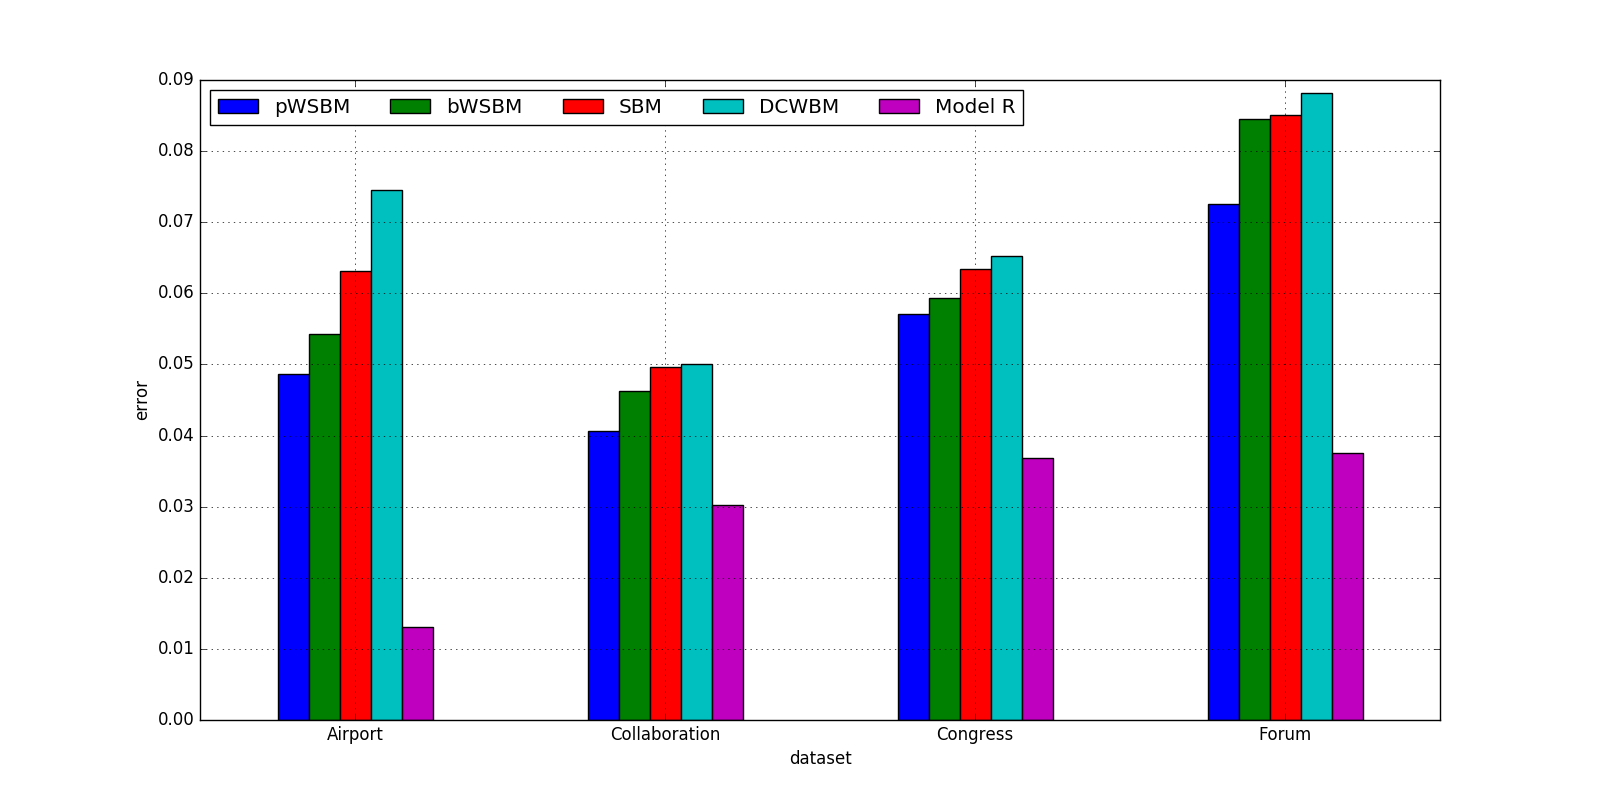
\includegraphics[width=1\textwidth]{link-weight-errors}
	\caption{
		The mean squared errors of 5 models on 4 datasets:
		Model R has lower error than every other model on every dataset.
		Every error value shown here is the mean error for the 25 trials in the experiment.
	}
	\label{fig:errors}
\end{figure*}
\begin{table*}[!htb]\centering
	\caption{
		The mean squared errors with standard deviations of 5 models on 4 datasets.
		Welch's t-test defines its p value as the Student's t-distribution cumulative density function $ p = 2 \int_{-\infty}^{-|t|} f(x) dx $.
	}
	\begin{tabularx}{\textwidth}{|c|X|X|X|X|X|c|c|} \hline \rowcolor{blue!30}
		Dataset & pWSBM & bWSBM & SBM & DCWBM & Model R & Reduction & p \\ \hline
		Airport & 0.0486 $ \pm $ 0.0006 & 0.0543 $ \pm $ 0.0005 & 0.0632 $ \pm $ 0.0008 & 0.0746 $ \pm $ 0.0009 & 0.013 $ \pm $ 0.001 & 73\% & 4.2e-66 \\ \hline
		Collaboration & 0.0407 $ \pm $ 0.0001 & 0.0462 $ \pm $ 0.0001 & 0.0497 $ \pm $ 0.0003 & 0.0500 $ \pm $ 0.0002 & 0.030 $ \pm $ 0.001 & 25\% & 9.1e-44 \\ \hline
		Congress & 0.0571 $ \pm $ 0.0004 & 0.0594 $ \pm $ 0.0004 & 0.0634 $ \pm $ 0.0006 & 0.0653 $ \pm $ 0.0004 & 0.036 $ \pm $ 0.003 & 35\% & 7.1e-35 \\ \hline
		Forum & 0.0726 $ \pm $ 0.0003 & 0.0845 $ \pm $ 0.0003 & 0.0851 $ \pm $ 0.0004 & 0.0882 $ \pm $ 0.0004 & 0.037 $ \pm $ 0.001 & 48\% & 4.2e-68 \\ \hline
	\end{tabularx}
	\label{tab:errors}
\end{table*}
In this section we compare Model R with the baseline models on every dataset.
Given the dataset,
we regard ModelRError (as well as BaselineError) as a random variable
so each trial generates an example of it.
We can do a t-test to justify the significance of the difference between the means of variables ModelRError and BaselineError.
The mean of a variable is not the same as the mean of a sample of the variable.
More specifically, a variable can generate two samples with different sample means,
therefore two samples with different means do not imply the two variables generating them have different means.
For each dataset, we do a t-test for the two variables where the null hypothesis is that the two variables have the same mean:
\begin{align*}
\overline{X_1} == \overline{X_2}
\end{align*}
where $ X_1 $ and $ X_2 $ are ModelRError and BaselineError and
where $ \overline{X} $ is the mean of variable X.
Welch's t-test defines its p value as the Student's t-distribution cumulative density function:
\begin{align*}
p = 2 \int_{-\infty}^{-|t|} f(x) dx
\end{align*}
The smaller p is, the more confidently we can reject the null hypothesis, i.e., accept that:
\begin{align*}
\overline{ModelRError} \neq \overline{BaselineError}
\end{align*}
Typically there is a domain specific threshold for p, e.g., 0.1 or 0.01. If p is smaller than the threshold we reject the null hypothesis.
We calculate the p value and also error reduction from baseline to Model R as:
\begin{align*}
Reduction = \frac{BaselineError - ModelRError}{BaselineError}
\end{align*}
The p value is almost 0 for all datasets and error reduction is significant,
shown in Table \ref{tab:errors}.
Model R has lower error than every other model on every dataset,
reducing error by 25\% to 73\% from the best baseline model - pWSBM.
The very low p values strongly indicate the error reduction is significant.
These results show that Model R outperforms pWSBM on all these datasets.
In our experiments, we have not observed any significant (more than 5\%)
prediction error increase or decrease when we change parameters around the values
we typically choose.
Overall, Model R has demonstrated a very high level of model robustness.

\subsection{Reproducibility}
In order to ensure the reproducibility of the experiment,
we specify the implementation details in this section:
\begin{itemize}
	\item Programming language: Python 3
	\item Python implementation: CPython 3.5
	\item Deep learning package: TensorFlow \cite{abadi2016tensorflow}
	\item Operating system: Ubuntu 16.10 64-bit
	\item Memory: 16 GB
	\item Processor: Intel Core i7-4770 CPU @ 3.40GHz
\end{itemize}
The program uses all 8 threads of the processor.
Each experiment takes about one hour to finish,
depending on the dataset and parameters in the learning algorithm.
The program is open-source under MIT license hosted on Github \footnote{https://github.com/yuchenhou/elephant}
so that everyone can use it without any restriction.

\section{Node embedding analysis}
The purpose of this section is to find out what knowledge Model R learns during training.
Our hypothesis is that the knowledge it learns consists of meaningful node embeddings where similar nodes (according to our own (human) semantics associated with the domain's entities) are close to each other in the node embedding space.
We make this hypothesis based on the following observations that Model R and the skip-gram model have similar architecture in their one-hot encoding input layer and linear embedding layer, and that the skip-gram model produces word embeddings where similar words are close to each other in the word embedding space.
Our goal is to verify this hypothesis by analyzing and visualizing the node embeddings produced by Model R in real world datasets from well understood domains to make the results obvious to most readers.

\subsection{Motivation}
Seeing the good performance of Model R, we are interested in this question: what exactly does Model R learn?
Even though Model R outperforms some of the latest link weight prediction techniques by a large margin, the knowledge it learns is not apparent.
We claim that Model R learns knowledge of nodes in the form of node embeddings from the known link weights and uses that knowledge to predict unknown link weights.
This claim is plausible and similar to the claim in the original word2vec paper \cite{mikolov2013linguistic}.
There have been several studies on word2vec focusing on the analysis and visualization of the word embeddings \cite{mikolov2013distributed} \cite{mikolov2013linguistic}.
These studies have provided strong evidences that the word embeddings learned by the skip-gram model represent meaningful knowledge about words.
However, we need to provide evidence that the node embeddings learned by Model R represent knowledge consistent with our understanding of the domain.
If we can have more in-depth study on those node embeddings similar to the studies on word embeddings, we can have a much better understanding of what Model R learns and why it performs well.

\subsection{Methods}
In order to perform node embedding analysis,
the experiment needs additional embedding logging and visualization methods.
The model trains on the datasets and produces node embeddings.
The visualizer reduces the dimension of the embeddings,
attaches domain metadata to the embeddings and produces the final visualization.
The visualization is then analyzed to confirm closeness of semantically-similar nodes.

\subsubsection{Datasets}
In order to verify the knowledge of nodes learned by the model is meaningful (agrees with our domain knowledge), the experiments use real world datasets from two well known domains:
\begin{itemize}
	\item Collaboration \cite{pan2012world}.	
	Nodes represent 226 nations on Earth, and each of the 20616 edges is weighted by the number of academic papers whose author lists include that pair of nations.
	This is the same dataset used in Section \ref{section:experiments} to evaluate the prediction error of Model R.
	\item MovieLens100K \cite{harper2015movielens}.
	This dataset is a recommendation dataset, and also a bipartite graph dataset.
	Nodes represent 1000 users and 1700 movies, and each of the 100000 edges is weighted by the rating score a user has given to a movie.
\end{itemize}
A snippet of MovieLens100K dataset is shown in Table \ref{tab:movielens100k} as an example.
\begin{table}[!ht]
	\centering
	\caption{A snippet of MovieLens100K dataset.}
	\begin{tabular}{ccc}  \hline \rowcolor{blue!30}
		User ID & Movie ID & rating \\ \hline
		196 & 272 & 3 \\ \hline
		186 & 302 & 3 \\ \hline
		22 & 377 & 1 \\ \hline
		244 & 51 & 2 \\ \hline
		166 & 346 & 1 \\ \hline
		... & ... & ... \\ \hline
	\end{tabular}
	\label{tab:movielens100k}
\end{table}

\subsubsection{Embeddings}
The model maps each node to a vector, or embedding, and it is these vectors that we will visualize and analyze.
Technically, these embeddings are the weights of the embedding layer of Model R shown in Figure \ref{fig:model-r}.

\subsubsection{Metadata}
The metadata provides domain specific information about the datasets necessary to verify the embeddings match our understanding about the specific domain. A snippet of MovieLens100K dataset metadata is shown in Table \ref{tab:movielens100kmeta} as an example.
\begin{table}[!ht]
	\centering
	\caption{A snippet of MovieLens100K dataset metadata.}
	\begin{tabular}{ccc} \hline \rowcolor{blue!30}
		Movie ID & Title & Release date \\ \hline
		1 & Toy Story & 01-Jan-1995 \\ \hline
		2 & GoldenEye & 01-Jan-1995 \\ \hline
		3 & Four Rooms & 01-Jan-1995 \\ \hline
		4 & Shanghai Triad & 01-Jan-1995 \\ \hline
		5 & Twelve Monkeys & 01-Jan-1995 \\ \hline
		... & ... & ... \\ \hline
	\end{tabular}
	\label{tab:movielens100kmeta}
\end{table}

\subsubsection{Model training}
The model training process is the same as the previous experiment,
with an extra step to log embedding layer weights.

\subsubsection{Embedding visualization}
The embedding visualization process plays an important role in the final knowledge representation.
This embedding visualization process has the following steps:
\begin{enumerate}
	\item Join the metadata and the embeddings on the node ID to attach the related information provided by the metadata to each node.
	\item Calculate the Euclidean distances between pairs of nodes.
	\item Dimensionality reduction through PCA (principal component analysis) on the embeddings to project these points from the high dimensional embedding space to a 2-dimensional space so that we can visualize them.
	\item Display all embeddings in an image, e.g., Figure \ref{fig:movies} and Figure \ref{fig:countries}.
\end{enumerate}

\subsection{Data analysis and visualization}
The experiment results meet our expectation - nodes more similar to each other (based on their semantics associated with the specific domain) have their corresponding points closer to each other in the embedding space.
The experiment process runs once for each of the two datasets: MovieLens100K and Collaboration.
We present the data analyses on a few well known cases and visualizations on the entire datasets as well.
The analysis for each dataset has the following steps:
\begin{enumerate}
	\item Select a well known reference node in the domain with two similar nodes that are easy to identify.
	\item Sort all nodes with respect to their distances to the reference.
	\item Verify that the distances from the two similar nodes to the reference node are much shorter than that of the median point.
\end{enumerate}
In this section, we perform data analysis on the experiment results for both datasets.

\subsubsection{MovieLens100K}
For this dataset, we select the movie ``Star Wars: The Empire Strikes Back" as the reference movie and the other two movies in the original Star Wars trilogy as the two similar movies, i.e., ``Star Wars: A New Hope" and ``Star Wars: Return of the Jedi".
Notice that we do not need to assume which attributes of a movie have the most influence in users' preferences for movies, because these two movies are similar to the reference movie in many attributes such as genre, actors, screenwriter, distributor and storyline.
The distances of a number of closest movies to the reference movie are shown in Table \ref{tab:movielens100k-distance}.
\begin{table}[!ht]\centering
	\caption{
		The distances of movies to the reference movie for MovieLens100K dataset.
	}
	\begin{tabular}{ccc} \hline \rowcolor{blue!30}
		Movie & Distance & Similarity \\ \hline
		The Empire Strikes Back (1980) & 0 & self (reference) \\ \hline
		Raiders of the Lost Ark (1981) & 0.012 & most similar \\ \hline
		... & ... & ... \\ \hline
		Star Wars (1977) & 0.047 & more similar \\ \hline
		Return of the Jedi (1983) & 0.063 & more similar \\ \hline
		... & ... & ... \\ \hline
		Children of the Revolution (1996) & 0.256 & median point \\ \hline
		... & ... & ... \\ \hline
		Tomorrow Never Dies (1997) & 0.295 & less similar \\ \hline
		Ayn Rand: A Sense of Life(1997) & 0.296 & less similar \\ \hline
		... & ... & ... \\ \hline
		101 Dalmatians (1996) & 0.335 & least similar \\ \hline
	\end{tabular}
	\label{tab:movielens100k-distance}
\end{table}
The data indicate that the distances from similar movies to the reference movie are much shorter than that from the median point.
The embeddings of all movies are shown in Figure \ref{fig:movies}.
\begin{figure*}[!ht]\centering
	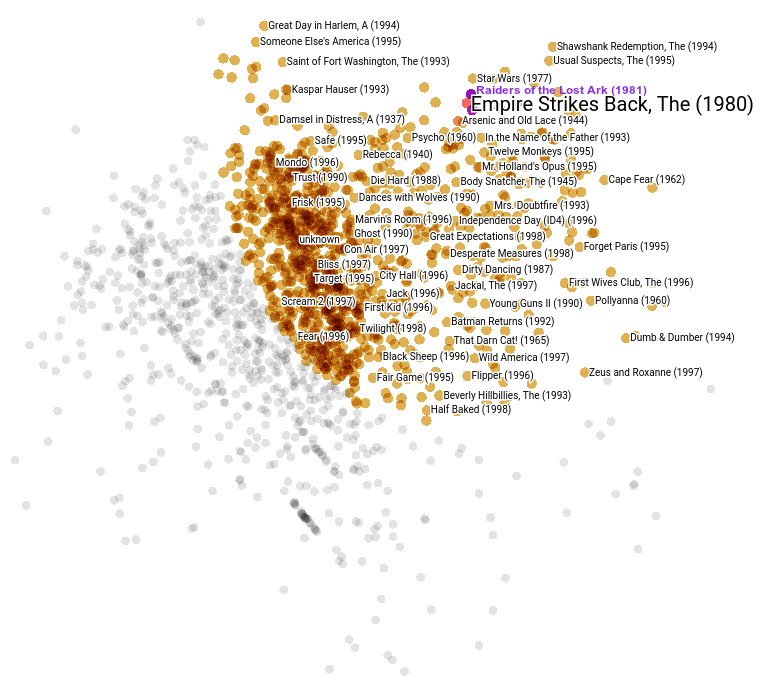
\includegraphics[width=0.8\textwidth]{movies-annotation}
	\caption{
		The embeddings of all movies in MovieLens100K dataset:
		``The Empire Strikes Back" is the reference movie, shown as a red node with bold font name.
		``Raiders of the Lost Ark" is the closest movie to the reference movie, shown as a purple node with purple name.
		A few other close movies are also shown as purple nodes.
		The image does not display names for many movies to avoid overlapping of the text.
		This embedding shows the overall distribution of movies where similar movies are closer to the reference movie.
	}
	\label{fig:movies}
\end{figure*}

\subsubsection{Collaboration}
For this dataset, we select the country United States as the reference country and two other countries with similar economy, education and culture backgrounds as the two similar countries: United Kingdom and Germany.
Notice that we assume economy, education and culture background have the most influence in international collaboration patterns.
The distances of a number of all countries to the reference country are shown in Table \ref{tab:countries-distance}.
\begin{table}[!ht]\centering
	\caption{
		The distances of countries to the reference country for Collaboration dataset.
	}
	\begin{tabular}{ccc} \hline \rowcolor{blue!30}
		Country & Distance & Similarity \\ \hline
		United States & 0 & self (reference) \\ \hline
		China & 0.216 & most similar \\ \hline
		... & ... & ... \\ \hline
		United Kingdom & 0.411 & more similar \\ \hline
		Germany & 0.483 & more similar \\ \hline
		... & ... & ... \\ \hline
		Jamaica & 29.531 & median point \\ \hline
		... & ... & ... \\ \hline
		Senegal & 31.018 & less similar \\ \hline
		Peru & 31.259 & less similar \\ \hline
		... & ... & ... \\ \hline
		Zimbabwe & 32.283 & least similar \\ \hline
	\end{tabular}
	\label{tab:countries-distance}
\end{table}
The data indicate that the distances from similar countries to the reference country are much shorter than that from the median point.
The embeddings of all countries are shown in Figure \ref{fig:countries}.
\begin{figure*}[!ht]\centering
	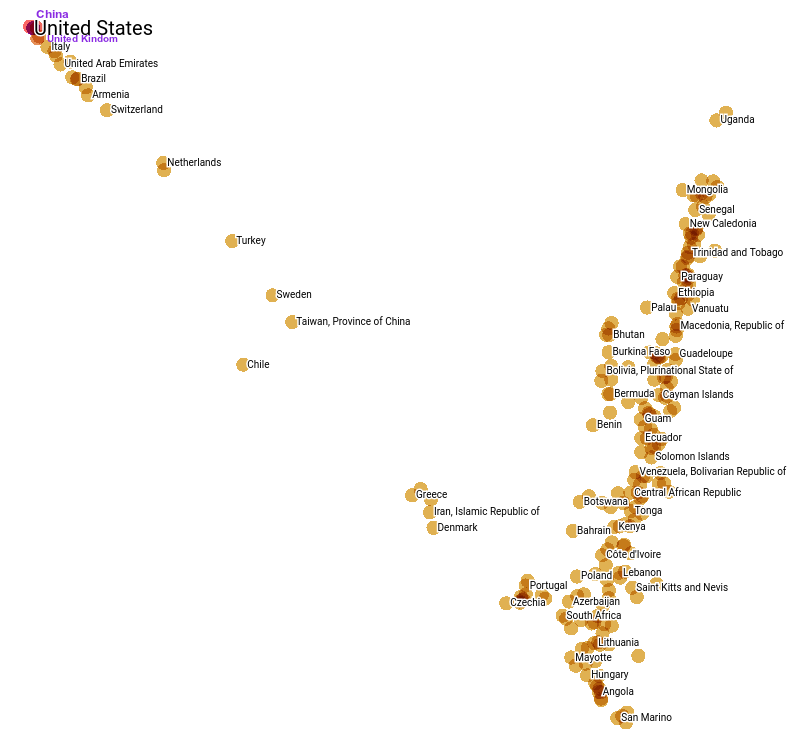
\includegraphics[width=0.8\textwidth]{countries-annotation-1}
	\caption{
		The embeddings of countries in Collaboration dataset:
		The United States is the reference country, shown as a red node with bold font name.
		China is the closest country to the reference country, shown as a purple node with purple name.
		A few other close countries are also shown as purple nodes.
		The image does not display names for many countries to avoid overlapping of the text.
		This embedding shows the overall distribution of countries where similar countries are closer to the reference country.
	}
	\label{fig:countries}
\end{figure*}

This chapter presents Model R, a deep learning model designed for the link weight prediction problem. Model R uses node embedding technique and feed forward architecture.
The scalability analysis shows Model R is more scalable with respect to the dataset size.
The experiments show that Model R has higher prediction accuracy than the state-of-the-art SBM and its derivatives.
A node embedding analysis with visualization provides strong evidence that Model R learns knowledge about nodes and represents this knowledge as node vectors.

\chapter{Model R in recommendation systems}
In this chapter, we study the application of Model R in
a special use case where the graph is a bipartite graph.
We put special attention on bipartite graphs because they are used to model relations between users and items/products in recommendation systems.
We provide an experimental evaluation of the performance of Model R, with comparison to four baseline approaches.

\section{Related work}
In this section,
we review existing deep learning methods in both content-based 
filtering and collaborative filtering.
We also clarify how our work differs from these related works.

\subsection{Content-based filtering methods}
Methods in this group extract information about an item from its content, 
i.e., the input of the neural network is a vector produced from the item's 
content (e.g., the audio of a song, the text of an article). Here are some 
examples:
\begin{itemize}
	\item One example is a music recommendation system 	\cite{van2013deep}. 
	It is a tag prediction system implemented with a convolutional neural net. 
	The input is the spectrogram vector of the audio of a song,
	and the output 	is the set of tags of the song (e.g., genre, instrumentation, tempo, mood).
	\item Another example is a multi-view recommendation system 	
	\cite{elkahky2015multi}. 
	It is a rating prediction system implemented with a fully connected 
	neural net.
	The input is the letter tri-gram vector of the text description of an item, 
	and the output is the rating.
	The letter tri-gram vector of a document is the count vector of all letter tri-grams in it, where each element in the vector is the number of appearances of a letter tri-gram. For example, the letter tri-grams of word ``recommendation'' are rec, eco, com, omm...
	\item A much more comprehensive example is a hierarchical Bayesian model 
	called collaborative deep learning \cite{wang2015collaborative}.
	This approach uses a stacked denoising autoencoder to extract information 
	from the bag-of-word vector of the text description of an item,
	and then uses the extracted information for rating prediction.
\end{itemize}
Similar to image recognition and speech recognition, these methods use deep 
learning to extract information about an entity from the content of the entity.
One of the limitations of content-based filtering is limited content analysis 
\cite{adomavicius2005toward}.
For example, if the items are articles addressing the same topic,
the badly written articles and well-written articles can have very similar 
textual content. In this case, a content-based system will fail to distinguish 
them and will give them similar ratings.
In this paper, we focus not on content-based filtering, but collaborative 
filtering (i.e., our technique does not access the contents of items).

\subsection{Collaborative filtering methods}
Methods in this group extract information about an item from its relations 
with other items,
and the neural net learns both a vector representation (embedding) of the relations and uses this vector to predict the rating.
These methods treat a list of items as a sentence of words 
(effectively reducing the problem to a natural language processing problem)  
and then apply the skip-gram model used in word2vec \cite{mikolov2013linguistic}:
\begin{itemize}
	\item An item similarity prediction example is item2vec 
	\cite{barkan2016item2vec} where purchases (lists of items) are 
	treated as sentences.
	\item Similar examples exist in graph mining, like deep walk 
	\cite{perozzi2014deepwalk} and node2vec \cite{grover2016node2vec}, 
	where a graph is sampled into walks (lists of nodes),
	and treated as sentences.
\end{itemize}
One drawback of these methods is that they fail to take advantage of 
the highly organized, regular and repeated structure in their relational data: 
relations between users and items (i.e., a user gives a numeric rating to an 
item) and relations between nodes of the same type (i.e., a source node connects to a 
destination node through a labeled link).
This structure is not exploited in natural language processing (i.e., for a neural net, words can simply show up in a sequence 
from a day-to-day conversation, in many flexible and unpredictable ways, with 
little structure or regularity).
Although syntax and semantics exist in natural languages, we have not seen any 
current neural network models taking advantage of these structures.
Our work differs from the above methods in that our technique uses a 
deep learning model designed to take advantage of the structure in the 
relational data and it is also able to predict a numeric attribute - the rating 
value.

\section{Problem}
The problem we consider in this section is collaborative rating prediction.
As an example of a collaborative rating prediction problem, consider 
a set of 6 users who give numeric ratings to a set of 3 items.
For each user, only a subset of their ratings are known; 
and we want to predict the unknown ratings.
The dataset for this example is shown in Table \ref{tab:ratings}.
For User[0], ratings to all 3 items are known; 
for User[1], ratings to Item[1] and Item[2] are known, 
but the rating to Item[0] is unknown; and so on.
Every unknown rating is marked as a question mark.
The task is to predict the unknown ratings.
\begin{table}[!htb]
	\centering
	\caption{Collaborative rating prediction problem example.}
	\begin{tabular}{cccc} \hline
		Ratings & Item[0] & Item[1] & Item[2] \\ \hline
		User[0] & 3       & 5       & 2 \\ \hline
		User[1] & ?       & 5       & 2 \\ \hline
		User[2] & 4       & 4       & 5 \\ \hline
		User[3] & 2       & 4       & ? \\ \hline
		User[4] & 5       & 5       & 4 \\ \hline
		User[5] & 4       & ?       & 4 \\ \hline
	\end{tabular}
	\label{tab:ratings}
\end{table}
Formally, a collaborative rating prediction problem is defined as follows:
\begin{itemize}
	\item Given: a 2-D array R[m][n], 
	where real number R[i][j] is the rating User[i] gives to Item[j], i $ \in [0, m-1] $, j $ \in [0, n-1] $,
	and p elements in R are unknown
	\item Task: predict all unknown elements in R to minimize mean absolute error (MAE), defined as
	\begin{align*}
	MAE = \frac{1}{p} \sum_{k = 1}^{p}|f_k - y_k|
	\end{align*}
\end{itemize}
where $ f_k $ is the predicted value, $ y_k $ is the true value, and p is the 
size of the test set.
Moreover, we define a user as the array of ratings they give to all items: 
\begin{align*}
User[i] = R[i]
\end{align*}

\section{Baseline solutions}
Among the many methods for the collaborative rating prediction problem,
the most prevalent one is the neighborhood-based collaborative filtering 
algorithm \cite{su2009survey}.
This algorithm also has several variants,
which we will use as baseline solutions.

\subsection{Algorithm}
The neighborhood-based collaborative filtering algorithm calculates each 
unknown R[i][j] as 
follows \cite{su2009survey}:
\begin{align*}
R[i][j] = c \sum_{k = 0}^{m-1} S(i, k) R[k][j]
\end{align*}
where S(i, k) is the similarity of User[i] and User[k] to be defined by each 
variant,
unknown R[k][j]'s are omitted and c is a normalizing factor:
\begin{align*}
c = \frac{1}{\sum_{k = 0}^{m - 1} |S(i, k)|}
\end{align*}
It is easy to understand the predicted rating R[i][j] as 
the sum of ratings each user gives to Item[j],
weighted by how similar each user is to the target user.
The algorithm can opt to use only a fixed number of users with highest 
similarities to the target user in the calculation, instead of using all users.

\subsection{Variants}
Each variant of the algorithm has a unique definition of the similarity 
function of User[i] and User[k]:
\begin{itemize}
	\item PCC: The Pearson correlation coefficient similarity, defined as 
	\cite{resnick1994grouplens}:
	\begin{align*}
	& S_{PCC}(x, y) \\
	=& \frac{\sum_{i \in I_{xy}}(R[x][i] - \overline{R[x]})(R[y][i] - 
		\overline{R[y]})}{\sum_{i \in I_{x}}(R[x][i] - \overline{R[x]})^2 
		\sum_{i 
			\in I_{y}}(R[y][i] - \overline{R[y]})^2 }
	\end{align*}
	where $ I_{x} $ is the set of items rated by User[x],
	$ I_{y} $ is the set of items rated by User[y],
	and	$ \overline{R[x]} $ is the average rating User[x] gives to all items,
	and $ I_{xy} $ is the set of items rated by both User[x] and User[y].
	PCC measures the linear correlation of two users.
	\item WPCC: The weighted PCC similarity, defined as 
	\cite{herlocker1999algorithmic}:
	\begin{align*}
	S_{WPCC}(x, y)=
	\begin{cases}
	\frac{|I_{xy}|}{T} S_{PCC}(x, y) & |I_{xy}| < T \\
	S_{PCC}(x, y) & otherwise
	\end{cases}
	\end{align*}
	where T is a threshold of number of items. 
	WPCC of two users differs from PCC only when the number of items rated by 
	both users (co-rated items) is less than the threshold. 
	When the difference occurs, fewer co-rated items results in less similarity 
	between the two users.
	\item SPCC: The sigmoid PCC similarity, defined as 	
	\cite{jamali2009trustwalker}:
	\begin{align*}
	S_{SPCC} (x, y)
	= \frac{S_{SPCC}(x, y)}{1 + exp(-\frac{|I_{xy}|}{2})}
	\end{align*}
	SPCC is similar to WPCC in the sense two users have lower similarity 
	if they have a smaller number of co-rated items.
	\item MPCC: The multi-level PCC similarity \cite{polatidis2016multi}. 
	This one is also similar to the previous ones but much more complex.
	MPCC essentially uses the PCC similarity measure, but increases it 
	based on the number of co-rated items between the two users,
	as long as the PCC similarity is sufficiently high.
	The more co-rated items, the larger the increase.
	But if the number of co-rated items or the PCC similarity is too low,
	then a similarity of zero is returned.
\end{itemize}


\section{Experiments}
We evaluated Model R and the baseline solutions experimentally,
and the results show that Model R achieved much lower prediction error than 
the baseline solutions.

\subsection{Datasets}
\label{datasets}
We evaluated Model R in the same settings used in a recent experimental 
evaluation of the baseline solutions \cite{polatidis2016multi} on four datasets:
\begin{itemize}
	\item ML100K: MovieLens100K \cite{harper2015movielens}. MovieLens 100,000 is a real dataset which contains 1682 movies, 943 users and 100,000 ratings. The data have been collected by the University of Minnesota and are associated with their online movie recommendation system. This particular dataset is one of the many that is publicly available from the University and has been widely used for offline experimental evaluation of collaborative filtering recommender system performance. The data in the dataset are in the form [userid] [itemid] [rating]. All the rating values are in the scale 1 to 5.
	\item ML1M: MovieLens1M \cite{harper2015movielens}. MovieLens 1 million is a real dataset which contains 4000 movies, 6000 users and 1,000,000 ratings. The data have been collected by the University of Minnesota and are associated with their online movie recommendation system. This particular dataset is one of the many that is publicly available from the University and has been widely used for offline experimental evaluation of collaborative filtering recommender system performance. The data in the dataset are in the form [userid] [itemid] [rating]. All the rating values are in the scale 1 to 5.
	\item EP: Epinions \cite{massa2007trust}. This is a publicly available dataset crawled from Epinions.com. It is a general product recommendation dataset. The data in the dataset are in the form [userid] [itemid] [rating]. All the rating values are in the scale 1 to 5. The dataset has 664,824 ratings from 49,290 users on 139,738 items.
	\item MT: MovieTweetings \cite{dooms2013movietweetings}. This is a publicly available dataset crawled from Twitter. It is a dataset consisting of movie ratings in the scale 0 to 10. The data in the dataset are in the form [userid] [itemid] [rating]. The dataset has 431,780 ratings from 39,363 users on 22,610 items.
\end{itemize}
The statistics of these datasets are summarized in Table \ref{tab:datasets-recommendation}.
\begin{table}[!ht]\centering
	\caption{
		The statistics of the graph datasets used in the recommendation system experiments.
	}
	\begin{tabular}{cccc}  \hline
		MovieLens100K & Users   & Items   & Ratings \\ \hline
		ML100K  & 1,000   & 1,700   & 100,000 \\ \hline
		MovieLens1M    & 6,000   & 4,000   & 1,000,000 \\ \hline
		Epinions      & 49,290  & 139,738 & 664,824 \\ \hline
		MT      & 39,363  & 22,610  & 431,780 \\ \hline
	\end{tabular}
	\label{tab:datasets-recommendation}
\end{table}

\subsection{Experiment process}
We do the same experiment for each dataset.
Each experiment consists of 25 independent trials.
In each trial, we split the dataset randomly into 3 subsets:
\begin{itemize}
	\item 70\% into training set
	\item 10\% into validation set
	\item 20\% into testing set
\end{itemize}
A larger or smaller validation set did not reduce the prediction error in the 
experiments.
We use mean absolute error (MAE) as the prediction performance metric.
For each trial, the model learns for several epochs.
In each epoch,
it learns on the training set,
predicts on the validation set,
and logs the validation error.
In order to reduce over-fitting,
the estimator stops learning when the validation error has not decreased for 3 
epochs.
At the end, the testing program lets the estimator predict on the test set 
and record its testing error as its prediction error on that dataset.
For each experiment, we report the mean of the errors from 25 trials.

\subsection{Experiment running time}
We record the mean number of epochs and training time needed for each experiment, shown in Table \ref{tab:time-recommendation}.
Model S with Model R embeddings runs faster than with node2vec embeddings on all four datasets, and faster than LLE embeddings on three of the four datasets.
\begin{table}[!htb]
	\centering
	\caption{
		The number of epochs and running time (seconds) of the experiment on four datasets.
	}
	\begin{tabular}{ccc} \hline \rowcolor{blue!30}
		Dataset & mean number of epochs & mean running time for each epoch (seconds) \\ \hline
		MovieLens100K & 10 & 5.647 \\ \hline
		MovieLens1M & 7 & 31.894 \\ \hline
		Epinions & 6 & 19.770 \\ \hline
		MovieTweetings & 6 & 16.584 \\ \hline
	\end{tabular}
	\label{tab:time-recommendation}
\end{table}

\subsection{Model prediction performance}
In our experiments, Model R's prediction error is 9\% to 18\% lower than the best baseline solution (i.e., MPCC) on all datasets, as shown in Table 
\ref{tab:rating-errors} and Figure \ref{fig:rating-errors}.
\begin{figure*}[!ht]\centering
	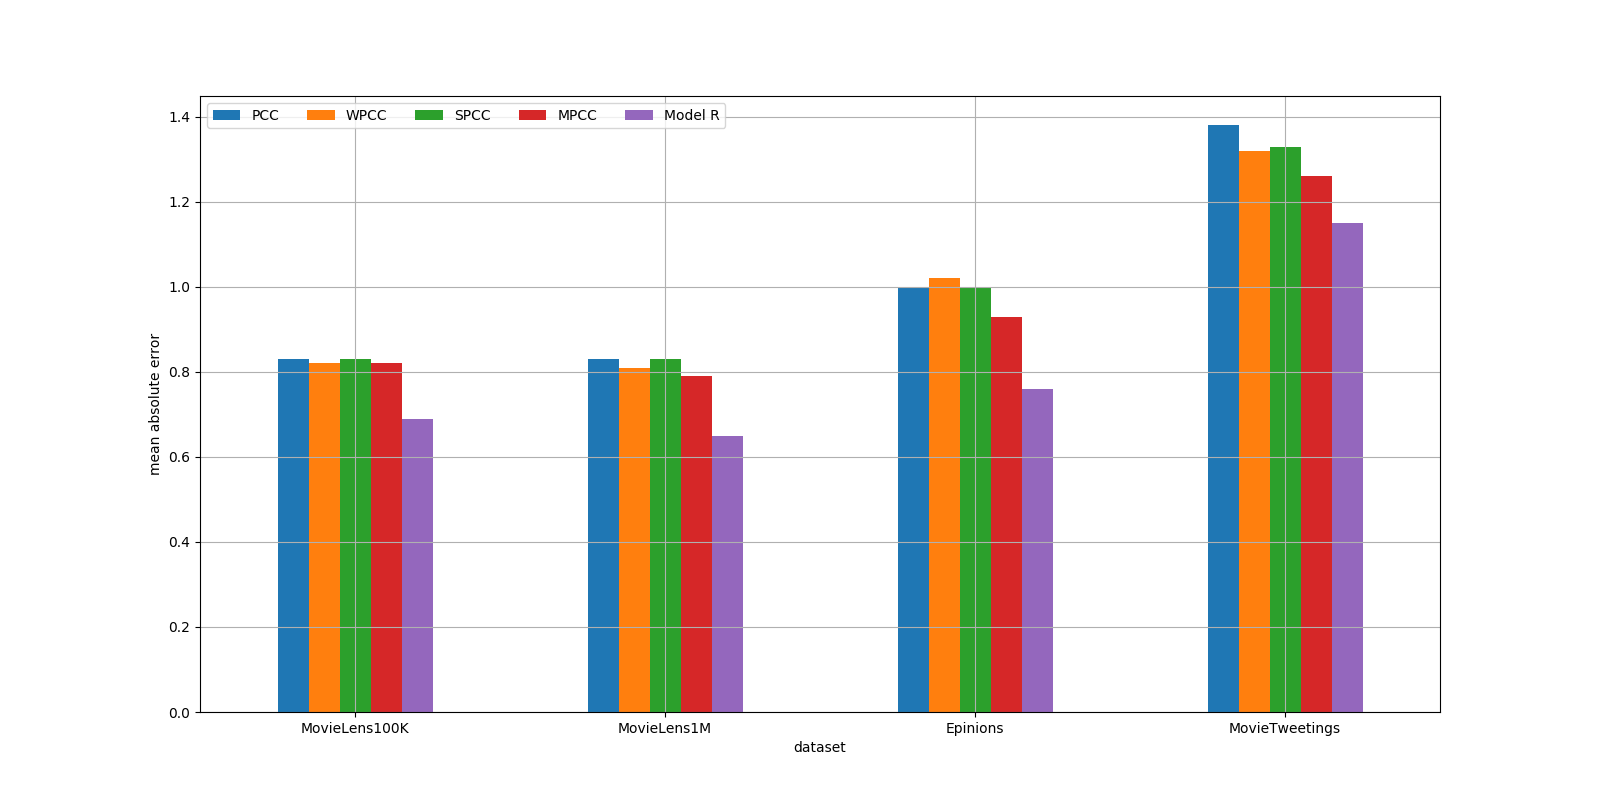
\includegraphics[width=1\textwidth]{rating-errors}
	\caption{
		The mean absolute errors of 5 models on 4 datasets:
		Model R has lower error than every other model on every dataset.
		Every error value shown here is the mean error for the 25 trials in the experiment.
	}
	\label{fig:rating-errors}
\end{figure*}
The error reduction from MPCC to Model R is calculated as:
\begin{align*}
\delta = \frac{MPCCError - ModelRError}{MPCCError}
\end{align*}
\begin{table}[!htb]
	\centering
	\caption{
		The comparison of prediction errors (measured by MAE).
		Model R's (represented by letter R) prediction error is 9\% to 18\%
		lower than the best baseline 
		solution (MPCC) on all datasets.
		Welch's t-test calculates its p value using the Student's t-distribution cumulative density function.
	}
	\begin{tabular}{cccccccl} \hline
		Dataset & PCC & WPCC & SPCC & MPCC & Model R & $ \delta $ & p \\ \hline
		MovieLens100K & 0.83 & 0.82 & 0.83 & 0.82 & 0.69 & 16\% & 6.7e-75 \\ \hline
		MovieLens1M & 0.83 & 0.81 & 0.83 & 0.79 & 0.65 & 18\% & 4.8e-48 \\ \hline
		Epinions & 1.00 & 1.02 & 1.00 & 0.93 & 0.76 & 18\% & 3.5e-64 \\ \hline
		MovieTweetings & 1.38 & 1.32 & 1.33 & 1.26 & 1.15 & 9\%  & 2.7e-63 \\ \hline
	\end{tabular}
	\label{tab:rating-errors}
\end{table}
Model R is also very robust in a wide range of parameter settings.
The robustness of performance against parameter changes on MovieLens100K dataset is shown in Table \ref{tab:robust}.
The results for other datasets are similar.
\begin{table}[!htb]
	\centering
	\caption{High robustness of Model R against parameter changes:
		The estimator maintains its prediction error in range [0.68, 0.73] for 
		a wide range of parameter settings. The batch size is the size of the 
		batch of samples used in a single gradient descent step.
		These experiments are on MovieLens 100K dataset with learning rate set 
		at 0.01.
	}
	\begin{tabular}{cccc}  \hline
		batch size & layer size & hidden layers \# & MAE \\ \hline
		16 & 16 & 2 & 0.714 \\ \hline
		16 & 16 & 8 & 0.710 \\ \hline
		16 & 64 & 2 & 0.687 \\ \hline
		16 & 64 & 8 & 0.706 \\ \hline
		64 & 16 & 2 & 0.703 \\ \hline
		64 & 16 & 8 & 0.724 \\ \hline
		64 & 64 & 2 & 0.703 \\ \hline
		64 & 64 & 8 & 0.713 \\ \hline
	\end{tabular}
	\label{tab:robust}
\end{table}
Model R shows that deep learning can be successfully applied to the collaborative rating prediction problem
and it can achieve higher prediction performance than  state-of-the-art collaborative filtering methods.
The model powered by Model R effectively learns complex and unobservable 
user and item attributes from simple and observable relations (i.e., users rate items).
The model learns both to map each entity to a vector, and to predict the rating using these vectors.

\chapter{Model R with pre-trained embeddings}
In this chapter, we introduce an extension of Model R which uses embeddings produced by a generic node embedding technique.
We evaluate this approach with three different node embedding techniques experimentally and compare its performance with stochastic block model and its derivatives.

\section{Observations and motivation}
We are interested in decoupling two learning processes (node embedding learning and link weight prediction learning) in Model R to generalize it and design a generic deep learning approach.
There are several other general purpose node embedding techniques such as Node2vec \citep{grover2016node2vec}.
So we want to investigate if the node embeddings produced by those general purpose node embedding techniques are better than node embeddings produced by Model R.
If we can decouple the two learning processes in Model R, we can substitute the node embedding with any other node embedding technique.
This plug-and-play idea, if it works, is very appealing because every time a new node embedding technique comes out, we can easily use the embeddings it produces in link weight prediction and see if it can improve the prediction performance.

\section{Approach}
We want to create a generic link weight prediction approach that uses the node embeddings produced by any node embedding technique.

\subsection{Embedding techniques}
As deep learning techniques become more powerful and standardized,
a key process of a domain-specific deep learning application
is mapping entities to vectors in an embedding space,
because a neural net needs vectors as inputs.
These vectors are called embeddings and this process is called embedding.
Embeddings are ubiquitous in deep learning,
appearing in natural language processing (embeddings for words),
graph mining (embeddings for nodes) and other applications.
Embedding techniques learn these vectors from relations between words and nodes.
A common goal of these techniques is to ensure that
similar entities are close to each other in the embedding space.

\subsubsection{Node2vec: node embedding with skip-gram model}
Node2vec is a node embedding technique similar to word embedding \citep{grover2016node2vec}.
This technique reduces the node embedding problem to the word embedding problem and then applies the word embedding technique.
The most important step in this technique is to sample random walks (node sequences) from a graph.
Each random walk follows a 2nd order random walk policy: given the current node in the walk is v, the previous node in the walk is t, the unnormalized transition probability $ p(x | v, t) $ to the next node x is
\[ p(x | v, t) = \alpha(t, x) w_{vx} \]
where $ w_{vx} $ is the weight of the link (v, x), and
\begin{equation*}
	\alpha(t, x) =
	\begin{cases}
		\frac{1}{p} &\text{if $d_{tx} = 0$}\\
		1 &\text{if $d_{tx} = 1$}\\
		\frac{1}{q} &\text{if $d_{tx} = 2$}\\
	\end{cases}
\end{equation*}
where $ d_{tx} $ is the unweighted shortest path length from t to x (which can only be one of \{0, 1, 2\}).
The Return Parameter p controls the probability of revisiting the previous node t in the walk. With small values of p, the walk tends to go backward during the sampling process.
The In-out Parameter q controls the probability of visiting a node further away from the previous node t in the walk.
With small values of q, the walk tends to go forward during the sampling process.
The remaining probability is distributed to visiting other nodes adjacent to t.
This process is a generalization of an earlier node embedding technique DeepWalk \citep{perozzi2014deepwalk}.
More specifically, DeepWalk is a special case of Node2vec where the inbound parameter p and outbound parameter q are both set to 1.
A graph has many walks, which can produce a dataset where each example is a (node, context-node) pair.
For example, given a walk in a social network of users \{John, Mary, James, Alice, Bob\}, we have the context of James \{John, Mary, Alice, Bob\}.
By reducing walks (sequences of nodes) to natural language sentences (sequences of words) and nodes to words,
this technique reduces the node embedding problem to the word embedding problem.
The final outcome is similar nodes have similar embeddings.

\subsubsection{Model R: node embedding supervised by link weights}
Model R not only learns to predict link weights,
but also has its own node embedding technique, shown in Section \ref{model-r}.
In fact, Model R produces its own node embeddings.
The Model R based node embedding technique is different from the skip-gram based Node2vec technique.
One advantage of the Model R based node embedding technique is that it takes advantage of the highly organized, regular and repeated structure in the relational dataset representing a graph, i.e., a source node connects to a destination node through one and only one weighted link.
The skip-gram model does not exploit this structure in natural language processing.

\subsubsection{LLE (locally linear embedding): nonlinear dimensionality reduction}
LLE is a member of the family of manifold learning approaches \citep{roweis2000nonlinear}.
This technique is not specifically designed for any embedding task, but for dimensionality reduction.
This technique comprises two steps.
The first step is linear approximation of data points in the original high dimensional space, an optimization process where the cost function is
\begin{align*}
cost(W) = \sum_i |X_i - \sum_jW_{ij}X_j|^2
\end{align*}
where each data point (high dimensional vector) $ X_i $ is linearly approximated by its k nearest neighbors $ X_j $'s, and the weight matrix W is the linear approximation parameter to be optimized.
The weight matrix $ W $ is determined by the intrinsic geometric properties of the neighborhoods instead of the coordinate system, therefore it obeys an important symmetry: $ W $ is invariant to rotations, scalings, and translations in the coordinate system.
The second step is reconstruction of data points in a new low dimensional space, an optimization process where the cost function is
\begin{align*}
cost(Y) = \sum_i |Y_i - \sum_jW_{ij}Y_j|^2
\end{align*}
where each data point (low dimensional vector) $ Y_i $ is linearly approximated by its k nearest neighbors $ Y_j $'s with the same weight matrix W produced in the previous linear approximation step. Now the new coordinates Y are the parameters to be optimized.
To apply this method, we use each row in the adjacency matrix of the graph as a data point in the high dimensional space, and then use LLE to map all rows to node embeddings in the low dimensional space.

\subsection{Model S: link weight prediction with node embeddings}
We introduce Model S, a neural net model that predicts a link weight using a pair of node embeddings (produced by any node embedding technique) as its input.
Model S is a generalization of Model R. More specifically, Model R is a special case of Model S when the pair of node embeddings is produced by itself.
\begin{figure}[ht]\centering
	\newcommand{\layersep}{1cm}
	\begin{tikzpicture}
	[->, shorten >=1pt,node distance=\layersep]
	\tikzstyle{every pin edge}=[shorten <=1pt]
	\tikzstyle{layer} = [rectangle, text centered, draw=black, fill=green!30]
	
	\node (input1) [layer, fill=red!30, pin={[pin edge={<-}]below:}] {direct activation layer};
	\node [below of=input1, xshift = -1cm] {input = (source node's embedding,};
	\node (input2) [layer, fill=red!30, pin={[pin edge={<-}]below:}, xshift = 4cm] {direct activation layer};
	\node [below of=input2, xshift = 1cm] {destination node's embedding)};
	
	\node (hidden2) [layer, above of=input1, xshift=2cm] {fully connected layer};
	\node (hidden3) [layer, above of=hidden2] {fully connected layer};
	
	\node (output) [layer, fill=blue!30, above of=hidden3, pin={[pin edge={->}]above:}] {fully connected layer};
	\node [above of=output] {output = link weight};
	
	\path (input1) edge (hidden2);
	\path (input2) edge (hidden2);
	\path (hidden2) edge (hidden3);
	\path (hidden3) edge (output);
	
	\end{tikzpicture}
	\caption{
		Model S with 1 input layer (red), 2 hidden layers (green), and 1 output layer (blue).
		The input layer has two channels: one channel for the source node and one channel for the destination node.
		Only layers and their connections are shown,
		while the units in each layer and their connections are not shown.
	}
	\label{fig:model-s}
\end{figure}

The approach uses the well-known deep learning techniques of back propagation \citep{rumelhart1988learning} and stochastic gradient descent \citep{lecun2012efficient} in model training.
Empirically, we use multiple hidden layers where each layer contains $ d = log_2(n) $ hidden units where d (as in dimension) is the number of units in each hidden layer and n is the dataset size.
We will vary the number of hidden layers to assess impact on performance.
This approach updates the model at each training step so Model S is an online learning method as long as the node embedding technique it depends on is also an online learning method (every embedding method we discussed in this section except LLE is an online learning method).
Therefore, by using an online embedding method, Model S can handle streaming graphs.

\section{Experiments}
We evaluate Model S experimentally with SBM with pWSBM as baselines,
and compare their prediction errors on several datasets.
We use three different techniques to produce node embeddings: node2vec, LLE and Model R.
The results show that Model S outperforms the baselines with all three embedding techniques on three out of four datasets.
Model S with Model R embedding technique performs the best on all four datasets. The experiments use four datasets described in Section \ref{datasets}.

\subsection{Experiment process}
We do the same experiment for each dataset.
All the link weights are normalized to the range [-1, 1] after applying a logarithm function.
As mentioned in previous section, Model S is suitable as a online learning method for steaming graphs so it scales nicely with dataset size.
Each experiment consists of 25 independent trials.
In each trial, we split the dataset randomly into 2 subsets:
\begin{itemize}
	\item 80\% into training set
	\item 20\% into testing set
\end{itemize}
We use mean squared error as the prediction performance metric.
The model learns for one epoch in each independent trial in order to simulate online learning scenario.
The testing program lets the estimator predict on the test set 
and record its testing error as its prediction error on that dataset.
For each experiment, we report the mean of the errors from 25 trials.

\subsection{Experiment running time}
We record the running time of training for three different embedding methods, shown in Table \ref{tab:time}.
Model S with Model R embeddings runs faster than with node2vec embeddings on all four datasets, and faster than LLE embeddings on three of the four datasets.
\begin{table}[!htb]
	\centering
	\caption{
		The comparison of running time (seconds) for three different embedding methods on four datasets.
	}
	\begin{tabular}{cccc} \hline
		Dataset & model-s (node2vec) & model-s (lle) & model-s (model-r) \\ \hline
		airport & 4.008 & 1.484 & 0.880 \\ \hline
		collaboration & 6.517 & 1.192 & 1.151 \\ \hline
		congress & 1.728 & 1.029 & 1.469 \\ \hline
		forum & 18.310 & 1.633 & 0.974 \\ \hline
	\end{tabular}
	\label{tab:time}
\end{table}

\subsection{Model prediction performance}
We evaluate the performance of Model S and compare it with a previously published performance evaluation of two baselines SBM and pWSBM on 4 datasets (Airport, Collaboration, Congress and Forum) \citep{aicher2014learning}.
We were not able to acquire an implementation for SBM or pWSBM so we did not do any performance evaluation on other datasets.
Model S's prediction performance is better than the baselines on 3 out of 4 datasets.
Among all Model S variants,
the one with Model R embedding technique performs the best,
as shown in Figure \ref{fig:weight-errors} and in Table \ref{tab:weight-errors}.

\begin{table}[!htb]
	\centering
	\caption{
		The comparison of prediction errors (measured by mean squared error).
		Model S performs better when using 3 different embedding techniques (LLE, Model R and node2vec) on 3 out of 4 datasets (Airport, Collaboration, Congress and Forum).
		Every error value shown here is the mean error for the 25 trials in the experiment.
	}
	\begin{tabular}{cccccc} \hline
		Dataset & pwsbm & sbm & model-s(node2vec) & model-s(lle) & model-s(model-r) \\ \hline
		airport & 0.0486 & 0.0632 & 0.0171 & 0.0170 & 0.0114 \\ \hline
		collaboration & 0.0407 & 0.0497 & 0.0614 & 0.0576 & 0.0327 \\ \hline
		congress & 0.0571 & 0.0634 & 0.0398 & 0.0402 & 0.0365 \\ \hline
		forum & 0.0726 & 0.0851 & 0.0312 & 0.0294 & 0.0298 \\ \hline
	\end{tabular}
	\label{tab:weight-errors}
\end{table}

\begin{figure}[ht] \centering
	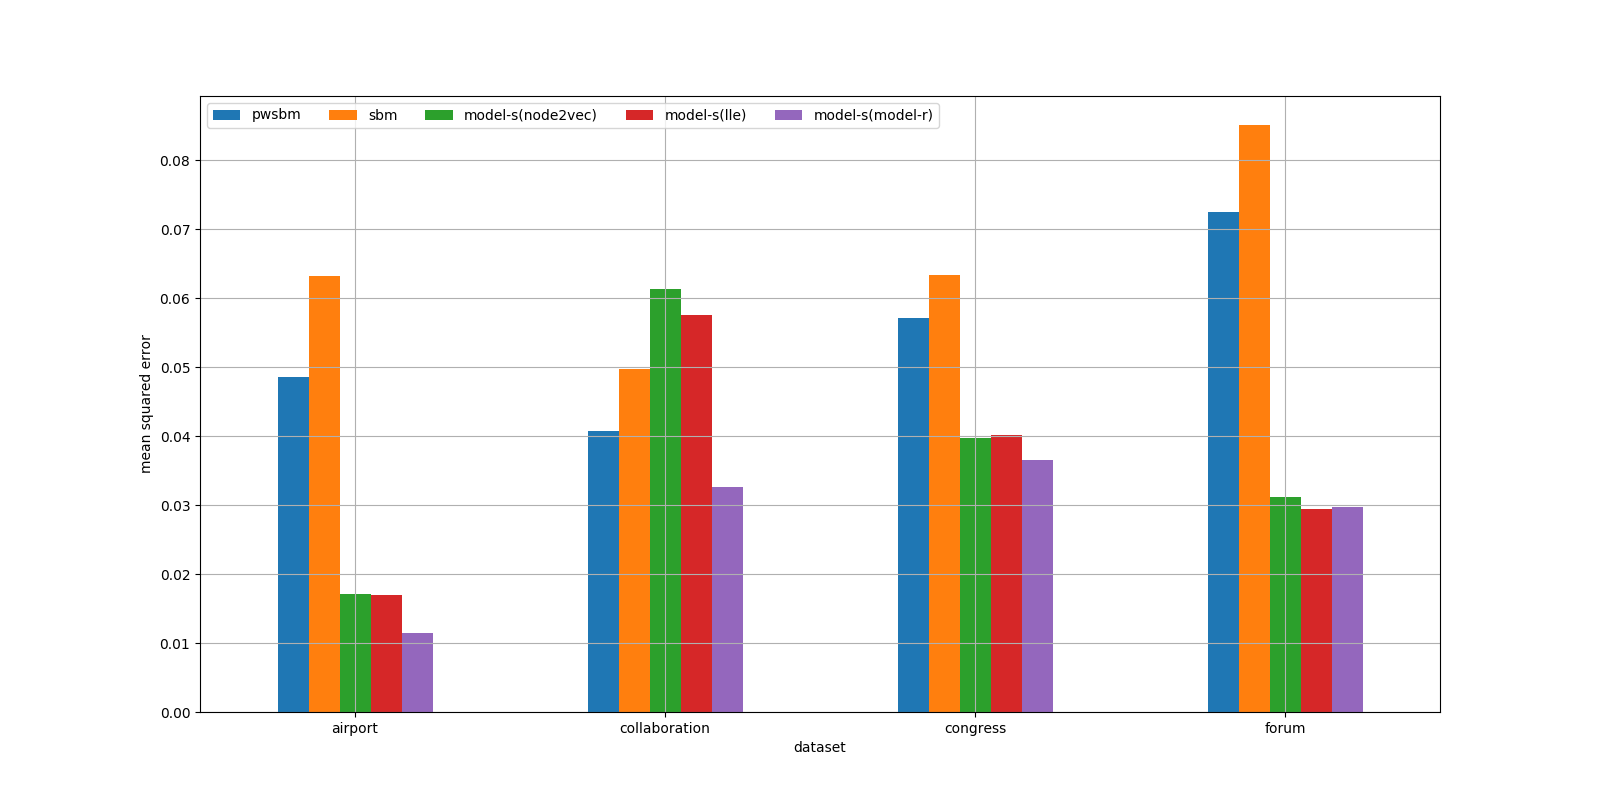
\includegraphics[width=1\linewidth]{weight-errors}
	\caption{
		Model S performs better when using 3 different embedding techniques (LLE, Model R and node2vec) on 3 out of 4 datasets (Airport, Collaboration, Congress and Forum).
		Every error value shown here is the mean error for the 25 trials in the experiment.
	}
	\label{fig:weight-errors}
\end{figure}
One obvious reason Model S can outperform baselines is higher level of flexibility.
SBM based approaches assume nodes within the same group are the same in terms of link weight distributions and the weight of every link follows a normal distribution.
Model S does not rely on these assumptions as it gives each node a unique description - the node embedding and it takes advantage of high flexibility of
layers of non-linear neural network units.
A possible reason why the Model S with Model R embedding outperforms the other two variants with node2vec and LLE embedding is that Model R embedding is specifically designed for the link weight prediction task.

\subsection{Model robustness}
In our experiments, Model S is robust against model parameter changes.
Adding or removing a hidden layer or several units in a hidden layer does not dramatically change the prediction error.
For example, when we set the number of hidden units in each hidden layer to the same constant value 20 and change the number of hidden layers,
the prediction error has little fluctuation (less than 10\%) when the number of hidden layers changes from 2 to 8,
as shown in Figure \ref{fig:robust-num-hidden-layers}.
\begin{figure}[ht] \centering
	\begin{subfigure}{0.49 \linewidth}
		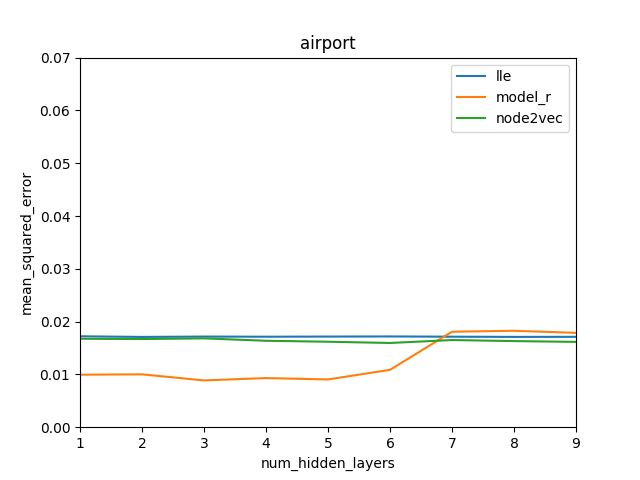
\includegraphics[width=\linewidth]{num_hidden_layers_airport}
		\caption{Evaluation on Airport dataset.}
	\end{subfigure}
	\begin{subfigure}{0.49 \linewidth}
		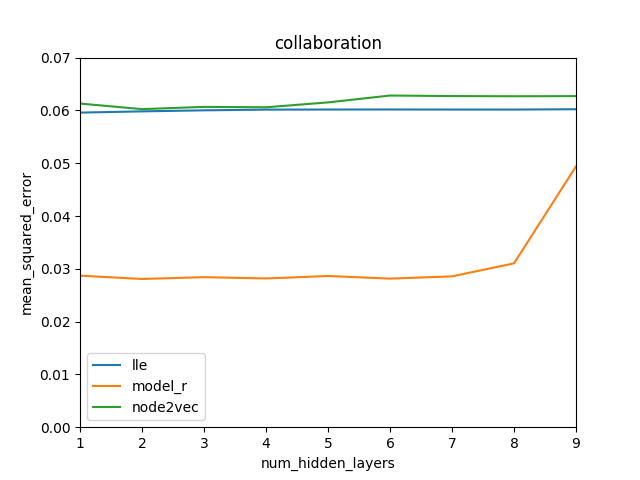
\includegraphics[width=\linewidth]{num_hidden_layers_collaboration}
		\caption{Evaluation on Collaboration dataset.}
	\end{subfigure}
	\begin{subfigure}{0.49 \linewidth}
		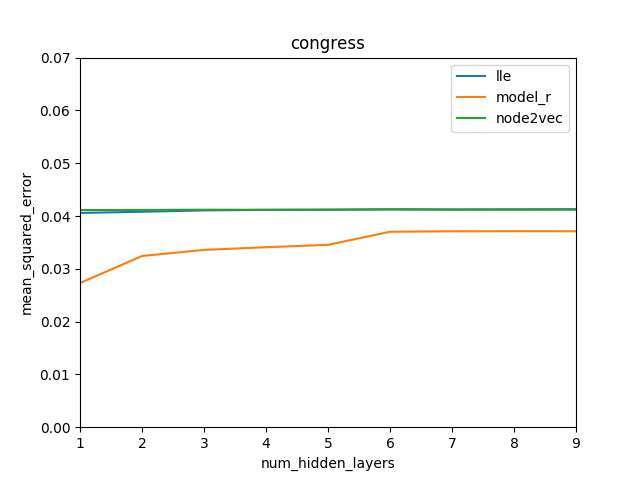
\includegraphics[width=\linewidth]{num_hidden_layers_congress}
		\caption{Evaluation on Congress dataset.}
	\end{subfigure}
	\begin{subfigure}{0.49 \linewidth}
		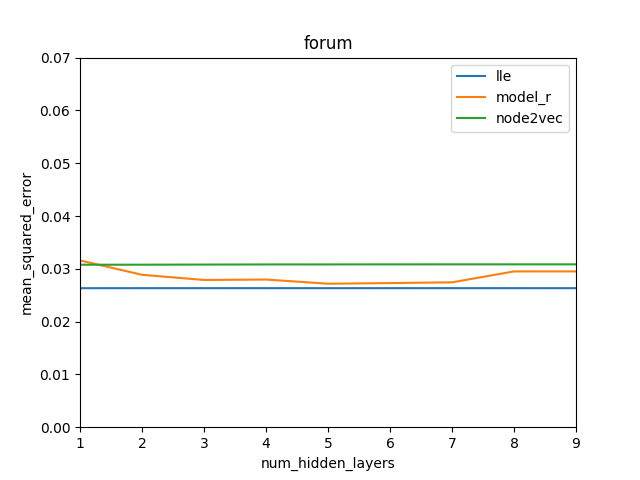
\includegraphics[width=\linewidth]{num_hidden_layers_forum}
		\caption{Evaluation on Forum dataset.}
	\end{subfigure}
	\caption{
		Model S is robust against changes of the model parameter number of hidden layers when using 3 different embedding techniques (LLE, Model R and node2vec) on datasets Airport, Collaboration, Forum and Congress.
	}
	\label{fig:robust-num-hidden-layers}
\end{figure}
Similar behavior is observed while varying other parameters, e.g., number of units per hidden layer.

Model S is a generalized deep learning approach to the graph link weight prediction problem based on general node embedding techniques.
In most cases, its prediction performance is better than the state-of-the-art non deep learning approaches SBM and pWSBM.
The Model R embedding performs the best among the different embeddings, which indicates that embeddings learned in the context of the task they will be used for can improve performance over generic embedding methods.

\chapter{Conclusion and future work}

\section{Conclusion}
Model R shows that deep learning can be successfully applied to the link weight prediction problem.
It effectively learns complex and unobservable node information (i.e., node vectors) from simple and observable relations between nodes (i.e., link weights),
and uses that information to predict unknown link weights.
Compared to SBM based approaches, Model R is significantly more accurate.
Two likely reasons are:
\begin{itemize}
	\item Higher level of discrimination for nodes:
	SBM based approaches do not differentiate nodes within the same group,
	and assume the weights of all links connecting two nodes from two groups
	follow the same distribution.
	Model R does not assume that,
	but gives every node a unique description - the node vector - so that
	it can have a more accurate description for every single node.
	\item Higher level of model flexibility:
	SBM based approaches assume the weight of every link follows
	a normal distribution.
	Model R does not assume that, but takes advantage of high flexibility of
	layers of non-linear neural network units,
	so that it can model very complex weight distributions.
\end{itemize}
Model R learns meaningful node embeddings where similar nodes (based on their semantics associated with the specific domain) are close to each other in the node embedding space.

Model S is the first generic deep learning approach to the link weight prediction problem based on node embeddings.
It requires an effective node embedding technique and works with various embedding techniques including
LLE, node2vec and the Model R.
In most cases, its prediction performance is better than the state-of-the-art non deep learning approaches SBM and pWSBM.
The Model R embedding performs the best among the different embeddings, which indicates that embeddings learned in the context of the task they will be used for can improve performance over generic embedding methods.

This work provides direct evidences that deep learning based embedding techniques are effective in two application domains beside natural language processing: recommender systems and graph mining.
We anticipate this new approach will provide effective solutions to more
graph mining tasks.

\section{Future work}
There are a few directions we would like to study in our future work on this model.

\subsection{Unified node embedding}

The first aspect is the mapping layer of Model R.
In the current model, the mapping layer contains two independent node dictionaries
to learn the node vectors.
During the learning stage, these two dictionaries learn to map the nodes to two spaces:
\begin{itemize}
	\item The source node dictionary maps nodes to source node space.
	\item The destination node dictionary maps nodes to destination node space.
\end{itemize}
A more compact approach is to have every node mapped to
one and only one node vector in both dictionaries,
as in the word2vec technique.
However, will this approach actually perform better?
Or does it depend on whether the graph is undirected or directed?
These are interesting questions to study in the future.

\subsection{Node embedding metrics}
An important direction for this work is to identify metrics for evaluating the learned node embeddings.
As embeddings are ubiquitous and valuable in deep learning and the popularity of deep learning is on the rise, we believe an important question is: what are good embeddings?
A direct answer can be: embeddings that match humans' perceptions of the nodes are good embeddings.
But humans' perceptions are, by nature, complicated and subjective.

As similar nodes should have their embeddings close to each other, a possible metric is the distances of the embeddings of similar nodes.
This is an obvious metric and also the one we tried to use intuitively for this work.
The distance measurement for embeddings is relatively easy but the similarity measurement for nodes is relatively hard.
One possible way to measure similarity is some type of statistics measurement of the behaviors of nodes.
For example, in recommender systems, it is natural to assume two users are very similar if they always give the same ratings to each one of the movies.
The challenge is this metric is not easy to measure if there are few movies rated by both users.
Another possible way to measure similarity is some type of measurement of the distance of their attribute vectors.
For example, the attribute vector of a user can be [age, gender, occupation, location] as exposed by the metadata.
In order for this measure to be useful, we need to know what attributes are the most relevant to users' movie preferences.

Node pairs with the same logical relation should have their embeddings exhibit the same spatial relation.
This one is less obvious and the logical relation measurement for nodes is hard.
In natural language processing, words can have very clear logical relations.
For example, (male, female) relation exists in word pairs such as [(gentleman, lady), (king, queen), (father, mother), (uncle, aunt)].
We have not identified any way to measure the logical relations for nodes.
For example, it is rather difficult to define any logical relation of two users or countries.

Good embeddings should produce good prediction performance, despite the type of node targeted for prediction.
This one is very obvious because eventually some other machine learning system should use these embeddings to do valuable predictions.
Therefore, good metrics should have positive correlation with prediction performance of the later stages of the deep learning system whose inputs are the embeddings.
This does not require any work with respect to the actual nodes but it is still hard to measure: some embeddings might work well on some models but not on other models, so it is hard to decide which model should be used as the evaluation reference.

\subsection{Complex graphs}
This direction is especially appealing for social network applications.
In particular, we want to handle graphs with node attributes.
Users can have labels like ``nationality", and real attributes like ``age".
One feasible approach is to append one unit for each of these attributes to the node vector.
For example, in order to better predict the rating a user gives to an article,
the model can append units at the mapping layer to receive a content vector 
mapped from the text of the article by another neural net.
The model can also append one unit for each numeric attribute of the user or 
item (e.g., the age of a user, the price of a product) at the mapping layer.
In this way, it will take advantage of not only relation data but also content 
data, and therefore make more accurate predictions.
Specifically, we consider to study how to use this technique to handle the 
following scenarios:
\begin{itemize}
	\item Handle links with string attributes: e.g., given a text message from 
	user A to user B (a link from A to B with a string attribute), the 
	estimator should extract knowledge of the users from the message content
	\item Handle links with logical implications: e.g., given a user has 
	written an article (a link from user to article with a ``write" attribute), 
	the estimator should extract knowledge of the user and the article from 
	this activity
	\item Handle nodes with rich attributes: e.g., given an article (a node 
	with a string attribute) or an image (a node with an image attribute), the 
	estimator should extract knowledge of the node from the article or image 
	content and integrate this knowledge with that extracted from links
\end{itemize}

\subsection{Large dynamic graphs}
A social network can have a large volume of links collected continuously by a
distributed system.
In the context of streaming data, new nodes and links appear in the stream, which requires the model to add new node embeddings without a complete retrain on the entire dataset.
A potential approach is to deploy an estimator to each computing node of
the distributed system and analyze a link stream there,
and let these estimators exchange their knowledge periodically.

The deep learning approach to link weight prediction presented in this thesis has potential impact on many real-world problems in industry.
For e-commerce, the enhancement in user-item rating prediction can make personalized product recommendation more effective and increase sales. For social media, the improvement on user interaction prediction can make friend recommendation more useful. We hope this work will see adoption in the industry and demonstrate its value with more real-world datasets.

\newpage

%*************** Epilogue *************************************
\let\WriteBookmarks\relax
%\pdfbookmark[0]{Bibliography}{thebibliography}

\bibliographystyle{plain}
\bibliography{references}



\end{document}
